% ============================================================
%  KCMamba: Kalman-Guided State-Space Model for Time Series Forecasting
%  ELTE Faculty of Informatics – TDK paper (37th OTDK)
%  Template: mcserep/elteikthesis v2.4  (MIT Licence)
% ============================================================
\documentclass[
    % parspace,
    % noindent,
    % nohyp,
    % twoside,
    % draft,
    % final,
]{elteikthesis}[2024/04/26]

% Document metadata
\title{KCMamba: Kalman-Guided Selective State-Space Model\\
       for Robust Time Series Forecasting}
\date{May 2026}

\author{András Kovács}
\degree{Computer Science BSc, Year 3}

\supervisor{Kristian Fenech Arian}
\affiliation{lecturer}

\university{Eötvös Loránd University}
\faculty{Faculty of Informatics}
\department{Department of Artificial Intelligence}
\city{Budapest}
\logo{elte_cimer_szines}

\PassOptionsToPackage{table}{xcolor}
\usepackage{colortbl}



% Long verbatim/command lines: enable automatic line breaking
\usepackage{fvextra}
\DefineVerbatimEnvironment{verbatim}{Verbatim}{breaklines=true,breakanywhere=true,fontsize=\footnotesize}

% Long \texttt{...} paths/identifiers should not overflow the margin
\setlength{\emergencystretch}{3em}

% Use case diagram (TikZ)
\usepackage{tikz}
\usetikzlibrary{shapes.geometric, positioning, fit, calc}

\addbibresource{bib/references.bib}

% ============================================================
\begin{document}
% ============================================================

\documentlang{english}

% ─── EXTERNAL COVER (OTDK requirement: "TDK-dolgozat" label + author name) ───
\begin{titlepage}
    \vspace*{\fill}
    \begin{center}
        {\Huge\bfseries TDK-dolgozat}\\[2.5cm]
        {\LARGE KCMamba: Kalman-Guided Selective\\[0.4em]
                State-Space Model for Robust\\[0.4em]
                Time Series Forecasting}\\[3cm]
        {\Large András Kovács}\\[0.5cm]
        {\large Computer Science BSc, Year 3}\\[2cm]
        {\large Eötvös Loránd University\\[0.3em]
                Faculty of Informatics}\\[0.8cm]
        {\large Budapest, May 2026}
    \end{center}
    \vspace*{\fill}
\end{titlepage}

% Internal title page (required: institution, faculty, dept, author, year, supervisor)
\maketitle

% Abstract
\chapter*{Abstract}
\addcontentsline{toc}{chapter}{Abstract}

This thesis presents \textbf{KCMamba} (Kalman Core-Attention Mamba),
a hybrid neural architecture that integrates a differentiable Kalman filtering
mechanism into the Mamba selective state-space model (SSM) for noise-robust
time series forecasting. The proposed architecture employs learned
$Q_\text{net}$, $R_\text{net}$, and $K_\text{net}$ subnetworks that adaptively
regulate the ratio of process and measurement noise, enabling the model to
behave as a passive predictor on clean data and as an active filter under noisy
conditions.

We conduct empirical evaluation on three public LTSF benchmarks
(Exchange-Rate, ETTh1, ETTh2) under synthetically injected noise
($\sigma \in \{0, 1, 3, 5\}$) and low data-availability regimes
(stride $\in \{1, 16\}$).

In the Exchange-Rate benchmark ($s=16$, 3-seed experiment), KCMamba's average
MSE degradation from $\sigma{=}0$ to $\sigma{=}5$ is $+1\,528\%$, compared
to $+28\,234\%$ for Fair Mamba, an $18.5\times$ stability gap; in the
hardest configuration ($s{=}16$, $\sigma{=}5$) KCMamba achieves MSE $1.41$
versus $22.72$ for Fair Mamba. The ablation study identifies the
$Q_\text{net}/R_\text{net}$ subnetworks as the primary source of robustness:
removing the learned $K$-gain increases degradation by $2.4\times$.

The thesis also describes the complete production software system: an
asynchronous, event-driven trading engine built in a hexagonal architecture,
a web-based dashboard, a backtesting framework, and a live Binance
trading adapter.

\cleardoublepage

% Table of Contents
\tableofcontents
\cleardoublepage

% ============================================================
%  MAIN TEXT
% ============================================================

% ============================================================
%  Chapter 1, Introduction
% ============================================================
\chapter{Introduction}
\label{ch:intro}

Time series forecasting is one of the most studied areas of applied machine
learning, partly because real-world data is almost always noisy.
Sensor dropouts, aggregation artefacts, and market microstructure noise all
degrade the signal-to-noise ratio, and models frequently struggle with this.
In the long-term forecasting (LTSF) setting the problem is harder still,
since a lookback window of length $L$ must support a prediction of the next $H$ steps,
where $H$ can exceed $L$~\cite{zhou2021informer}.

\section{Motivation}

Transformer-based models~\cite{zhou2021informer,wu2021autoformer} and the
Mamba SSM~\cite{gu2021s4,gu2023mamba} address data-quality issues through
implicit generalisation, relying on the model to learn around the noise.
This works on clean data, but there is no guarantee that the robustness
transfers to noisy regimes.

The Kalman filter~\cite{kalman1960new} takes a different route: it builds an
\emph{explicit} model of process noise ($Q$) and measurement noise ($R$), and
derives a gain $K$ from their ratio to decide how much to trust the current
measurement versus the prior state.
The \textbf{KCMamba} architecture presented in this thesis is built on
this principle. That inductive bias, if embedded in a neural network,
may help in noisy conditions.

\section{Research Questions}

Three questions are investigated: (1)~is KCMamba competitive on clean data
against standard LTSF models; (2)~how much MSE degradation do models suffer
under synthetically injected noise ($\sigma \in \{0, 1, 3, 5\}$);
and (3)~which architecture generalises better under scarce training data
(stride $\in \{1, 16\}$).

\section{Contributions}

The thesis makes five concrete contributions.
The \textbf{KCMamba} architecture embeds learned $Q_\text{net}$,
$R_\text{net}$, $K_\text{net}$ subnetworks inside a differentiable Kalman
filter, with a parallel prefix-scan GPU implementation for the recursion.
Measurements show that the learned $K$ genuinely adapts to noise:
$K \approx 0{.}71$ at $\sigma=0$ (passive pass-through) and
$K \approx 0{.}07$ at $\sigma=5$ (strong filtering).

Benchmark results on three datasets (Exchange-Rate, ETTh1, ETTh2) show
that Fair Mamba degrades by $28\,234\%$ under noise, whereas KCMamba
degrades by only $1\,528\%$ ($18.5\times$ smaller degradation).
The long-sequence analysis ($T \in \{96,192,336,512\}$, ETTm1 and
Exchange) confirms KCMamba's advantage at longer contexts:
at $T{=}336$, $\sigma{=}1$ it achieves $31.7\%$ lower MSE than LSTM
($0.502$ vs $0.735$); at $T{=}512$, $\sigma{=}3$, KCMamba scores $0.773$
while Fair Mamba scores $2.121$. On ETTm1 at $\sigma{=}3$ KCMamba is
the only model whose MSE monotonically decreases with sequence length
($0.673 \to 0.466$, $-31\%$, $T{:}\,96 \to 512$).
In the stride $\times$ sequence-length sweep ($s \in \{1,16\}$,
$T \in \{192,336,512\}$), at $s{=}16$, $\sigma{\geq}3$,
Fair Mamba's MSE rises to $8.1$--$8.5$ while KCMamba stays at $1.1$--$1.3$.
All experiments are accompanied by an open-source Python/PyTorch/CUDA
implementation integrated into an asynchronous live-trading system.

\section{Thesis Structure}

Chapter~\ref{ch:irodalom} reviews the Kalman filter, SSMs, and the
LTSF literature.
Chapter~\ref{ch:architektura} describes the KCMamba architecture and
its mathematical underpinnings.
Chapter~\ref{ch:kiserletek} presents the experimental setup and results.
Chapter~\ref{ch:implementacio} covers the implemented software system.
Chapter~\ref{ch:osszegzes} draws conclusions and discusses future work.

\cleardoublepage

% ============================================================
%  Chapter 2, Related Work
% ============================================================
\chapter{Related Work}
\label{ch:irodalom}

\section{The Kalman Filter and Its Extensions}
\label{sec:kalman}

The Kalman filter~\cite{kalman1960new} is the minimum-variance, unbiased, linear
estimator for systems whose state $x_t \in \mathbb{R}^n$ evolves according to
a linear dynamical model perturbed by Gaussian noise:
\begin{align}
    x_t &= F x_{t-1} + w_t, & w_t &\sim \mathcal{N}(0, Q), \label{eq:kf_process}\\
    y_t &= H x_t   + v_t,   & v_t &\sim \mathcal{N}(0, R), \label{eq:kf_measure}
\end{align}
where $F$ is the state-transition matrix, $H$ the observation matrix,
$Q \in \mathbb{R}^{n \times n}$ the process-noise covariance, and
$R \in \mathbb{R}^{m \times m}$ the measurement-noise covariance. The filter
operates in two alternating half-steps.
In the prediction step (time update), before the measurement $y_t$ arrives,
the filter propagates the state estimate and the error covariance forward
in time:
\begin{align}
    \hat{x}_{t|t-1} &= F \hat{x}_{t-1|t-1}, \label{eq:kf_predict_x}\\
    P_{t|t-1}       &= F P_{t-1|t-1} F^\top + Q, \label{eq:kf_predict_P}
\end{align}
where $P_{t|t-1} \in \mathbb{R}^{n \times n}$ is the predicted error
covariance. A large $P_{t|t-1}$ indicates high prediction uncertainty;
a large $Q$ means the system state changes rapidly and unpredictably.

In the correction step (measurement update), once the observation $y_t$
arrives, the filter corrects its estimate by the
\emph{innovation} $e_t = y_t - H\hat{x}_{t|t-1}$, weighted by the Kalman
gain $K_t$:
\begin{align}
    K_t           &= P_{t|t-1} H^\top \bigl(H P_{t|t-1} H^\top + R\bigr)^{-1},
                     \label{eq:kalman_gain}\\
    \hat{x}_{t|t} &= \hat{x}_{t|t-1} + K_t e_t, \label{eq:kalman_update}\\
    P_{t|t}       &= (I - K_t H)\,P_{t|t-1}. \label{eq:kf_update_P}
\end{align}
Equation~\eqref{eq:kalman_gain} encodes the fundamental noise-balance
intuition. When the measurement noise $R$ is large relative to the predicted
covariance $H P_{t|t-1} H^\top$, the denominator dominates and $K_t \to 0$:
the filter distrusts the observation and relies on its prior state. When $R
\to 0$, $K_t \to H^{-1}$ and the observation nearly overwrites the state
entirely.

For the scalar case ($F = H = 1$), the gain simplifies to
\begin{equation}
    K_t = \frac{P_{t|t-1}}{P_{t|t-1} + R}.
    \label{eq:kalman_gain_scalar}
\end{equation}
Under steady-state conditions the error covariance $P_{t|t-1}$ converges to a
fixed value $\bar{P}$, and the steady-state gain depends only on the ratio
$Q/R$: a high process noise relative to measurement noise drives $K$
towards~1 (trust the measurement), while a low $Q/R$ ratio drives $K$
towards~0 (trust the model). This $Q/(Q+R)$ ratio is the structural basis
for the KCMamba gain computation (Section~\ref{sec:kalman_gain}).

\subsection{Learned Kalman Filters}

In the neural Kalman literature, the matrices $F, H, Q, R$ are parameterised
by neural networks~\cite{krishnan2015deep,fraccaro2017disentangled}.
The \emph{Deep Kalman Filter}~\cite{krishnan2015deep} allows non-linear
transitions, and the \emph{Kalman Variational Autoencoder}~\cite{fraccaro2017disentangled}
learns disentangled representations of latent states.
KCMamba builds on these ideas but operates as a sequence forecaster rather
than as an autoencoder.

\section{State Space Models}
\label{sec:ssm}

\subsection{S4}

S4~\cite{gu2021s4} reformulates a sequence model as a parameterised ordinary
differential equation (ODE) over a latent state $h(t) \in \mathbb{R}^N$:
\begin{align}
    h'(t) &= A h(t) + B u(t), \label{eq:s4_continuous}\\
    y(t)  &= C h(t). \label{eq:s4_output}
\end{align}
Here $u(t)$ is the scalar input, $A \in \mathbb{R}^{N \times N}$ is the
state matrix, and $B, C \in \mathbb{R}^N$ are the input and output projections.
The critical insight of Gu et al.\ is that $A$ can be initialised as the
\emph{HiPPO} (High-order Polynomial Projection Operator) matrix, which is
designed to compress the history of $u$ into the current state $h(t)$ with
optimal polynomial approximation. This initialisation avoids the
vanishing-gradient problem that plagues vanilla RNNs over long sequences,
since the HiPPO structure preserves information from the distant past without
exponential decay.

To apply the model to discrete sequences the continuous system is discretised
with step size $\Delta$ using the zero-order hold (ZOH) rule:
\begin{align}
    h_t &= \bar{A} h_{t-1} + \bar{B} u_t, \label{eq:s4_discrete_h}\\
    y_t &= C h_t, \label{eq:s4_discrete_y}
\end{align}
where $\bar{A} = e^{\Delta A}$ and $\bar{B} = (e^{\Delta A} - I)A^{-1}B$.
Because $\bar{A}$ is diagonal in the frequency domain the entire convolution
$y = \bar{C} * u$ can be computed as a single element-wise product after an
FFT, reducing sequence-level complexity to $O(T \log T)$.

A fundamental limitation of S4 is that $A$, $B$, $C$, and $\Delta$ are
\emph{input-independent}: the same learned parameters are applied at every
time step regardless of the input content. The model therefore cannot adapt
its memory or forgetting behaviour in response to what it actually observes
in the current sequence.

\subsection{Mamba}

Mamba~\cite{gu2023mamba} addresses this limitation directly by making the
state-space parameters \emph{input-dependent}. The matrices $B$, $C$, and the
time step $\Delta$ are no longer fixed scalars but functions of the current
input $u_t$:
\begin{align}
    B_t      &= \mathrm{Linear}(u_t),  \\
    C_t      &= \mathrm{Linear}(u_t),  \\
    \Delta_t &= \mathrm{softplus}\bigl(\mathrm{Linear}(u_t) + \delta_\mathrm{bias}\bigr).
\end{align}
The time step $\Delta_t$ determines the discrete transition matrices
$\bar{A}_t = e^{\Delta_t A}$, $\bar{B}_t = (\bar{A}_t - I) A^{-1} B_t$.
This mechanism, called the \emph{Selective State Space} (S6) layer, lets the
model selectively remember or forget content at each step. When
$\Delta_t \to 0$ the state barely changes ($\bar{A}_t \approx I$),
preserving memory. When $\Delta_t$ is large the state is updated strongly,
discarding older information.

The input-dependent parameters break the global convolution trick that made
S4 efficient, because there is no longer a single kernel to FFT. Gu and Dao
solve this with a \emph{hardware-efficient parallel scan} (the Blelloch
prefix-scan algorithm), applied on the GPU's SRAM to avoid expensive
high-bandwidth memory round-trips. The scan runs in $O(\log T)$
synchronisation steps on $T$ parallel threads, achieving $O(T)$ total
work and $O(T)$ memory while avoiding the sequential bottleneck of recurrent
models.

\subsection{Fair Mamba}

The comparison baseline, referred to as ``Fair Mamba'', is a channel-wise Mamba
with identical hyperparameters and training protocol as KCMamba. The ``fair''
label means the parameter budget and data are identical, so any difference in
results comes solely from the architecture.

\section{Long-Term Time Series Forecasting}
\label{sec:ltsf}

\subsection{Problem Formulation}

Long-term time series forecasting (LTSF) considers an input window
$\mathbf{X} = (x_1, \ldots, x_L) \in \mathbb{R}^{L \times d}$ of $L$
historical steps across $d$ channels, and requires producing a prediction
$\hat{\mathbf{X}} = (\hat{x}_{L+1}, \ldots, \hat{x}_{L+H}) \in \mathbb{R}^{H \times d}$
for the next $H$ steps. The objective is to minimise the normalised mean
squared error
\begin{equation}
    \mathrm{MSE} = \frac{1}{H d}
        \sum_{h=1}^{H} \sum_{j=1}^{d}
        \frac{(x_{L+h,j} - \hat{x}_{L+h,j})^2}{\mathrm{Var}(x_{\cdot,j})},
    \label{eq:mse}
\end{equation}
where normalisation by the per-channel variance makes results comparable
across datasets with different scales. The \emph{long-term} qualifier refers
to the common regime $H \geq L$ or $H$ comparable to $L$: the model must
extrapolate well beyond the lookback window, which is substantially harder
than short-term forecasting where $H \ll L$.

\subsection{Reference Models}

\emph{Informer}~\cite{zhou2021informer} was the first Transformer variant
specifically designed for long-term forecasting. Standard self-attention has
$O(L^2)$ time and memory complexity, which becomes prohibitive for long input
windows. Informer addresses this with \emph{ProbSparse attention}: it
identifies the $O(\log L)$ most informative query positions via a KL-divergence
estimate, reducing complexity to $O(L \log L)$. A distilling operation
halves the sequence length between encoder layers so the model can handle
lookback windows of several thousand steps.

\emph{Autoformer}~\cite{wu2021autoformer} decomposes each series into a
trend component (estimated with a moving-average kernel) and a seasonal
residual, applying the Transformer only to the residuals. Rather than
dot-product attention it uses an \emph{Auto-Correlation} mechanism: it
identifies the lag $\tau$ maximising the autocorrelation of the query
signal and aggregates values at those lag offsets. The resulting mechanism
is $O(L \log L)$ via FFT and provides an inductive bias suited to periodic
data.

\emph{DLinear}~\cite{zeng2023transformers} discards all of this complexity
and applies a single linear layer to each lookback window to produce the
forecast, optionally after trend-seasonal decomposition. Despite its
simplicity, DLinear matched or outperformed many Transformer variants on
standard benchmarks, demonstrating that architectural complexity is not
always necessary for good forecasting performance. It remains a relevant
baseline because any new model must justify its additional overhead relative
to this linear reference.

\subsection{Datasets}
\label{sec:datasets}

The Exchange-Rate dataset~\cite{lai2018modeling} contains eight foreign exchange
rates sampled daily from 1990 to 2016, giving 7\,588 time steps per channel.
Exchange-rate data has near-unit-root dynamics: each daily increment is
close to a random walk with very little mean reversion. This makes it a
challenging benchmark for autoregressive models, and a natural setting
for evaluating the Kalman structure where the signal-to-noise ratio is
intrinsically low.

ETTh1 and ETTh2~\cite{zhou2021informer} are both collected from
Chinese transformer stations, recording hourly electricity load and oil
temperature for two years (17\,420 steps, $d=7$ channels). ETTh1 has a
clear daily periodicity, while ETTh2 is noisier and more irregular. The two
datasets provide contrasting difficulty levels for noise-robustness
evaluation.

\section{Noise Robustness}
\label{sec:robustness}

The noise sensitivity of time series models is rarely studied in
a systematic way. PatchTST~\cite{nie2022patchtst} indirectly improves noise
tolerance through patch tokenisation, but robustness is not its primary goal.

In this work the evaluation protocol is:
$\tilde{x}_t = x_t + \varepsilon_t$,
$\varepsilon_t \sim \mathcal{N}(0, \sigma^2 I)$, $\sigma \in \{0, 1, 3, 5\}$.
Both training and test sets are corrupted with the same $\sigma$, so this
is uniform data-quality degradation, not a domain-shift scenario.

\cleardoublepage

% ============================================================
%  Chapter 3, KCMamba Architecture
% ============================================================
\chapter{The KCMamba Architecture}
\label{ch:architektura}

\section{Overview}

KCMamba (Kalman Core-Attention Mamba) is a hybrid neural time-series
model that embeds a differentiable, content-dependent Kalman filter layer into
the Mamba SSM~\cite{gu2023mamba}.
Instead of using a fixed forgetting factor $A$, the model
learns a gain $K$ from the current input and uses it to decide how much to trust
the new measurement versus the prior state.

The model has two levels: the base processing unit is a
\texttt{KCMambaBlock} (content-dependent Kalman filtering and state update),
stacked into a \texttt{KCMambaStack} of $N$ sequential blocks with a
cross-attention layer at the top.

\begin{figure}[H]
  \centering
  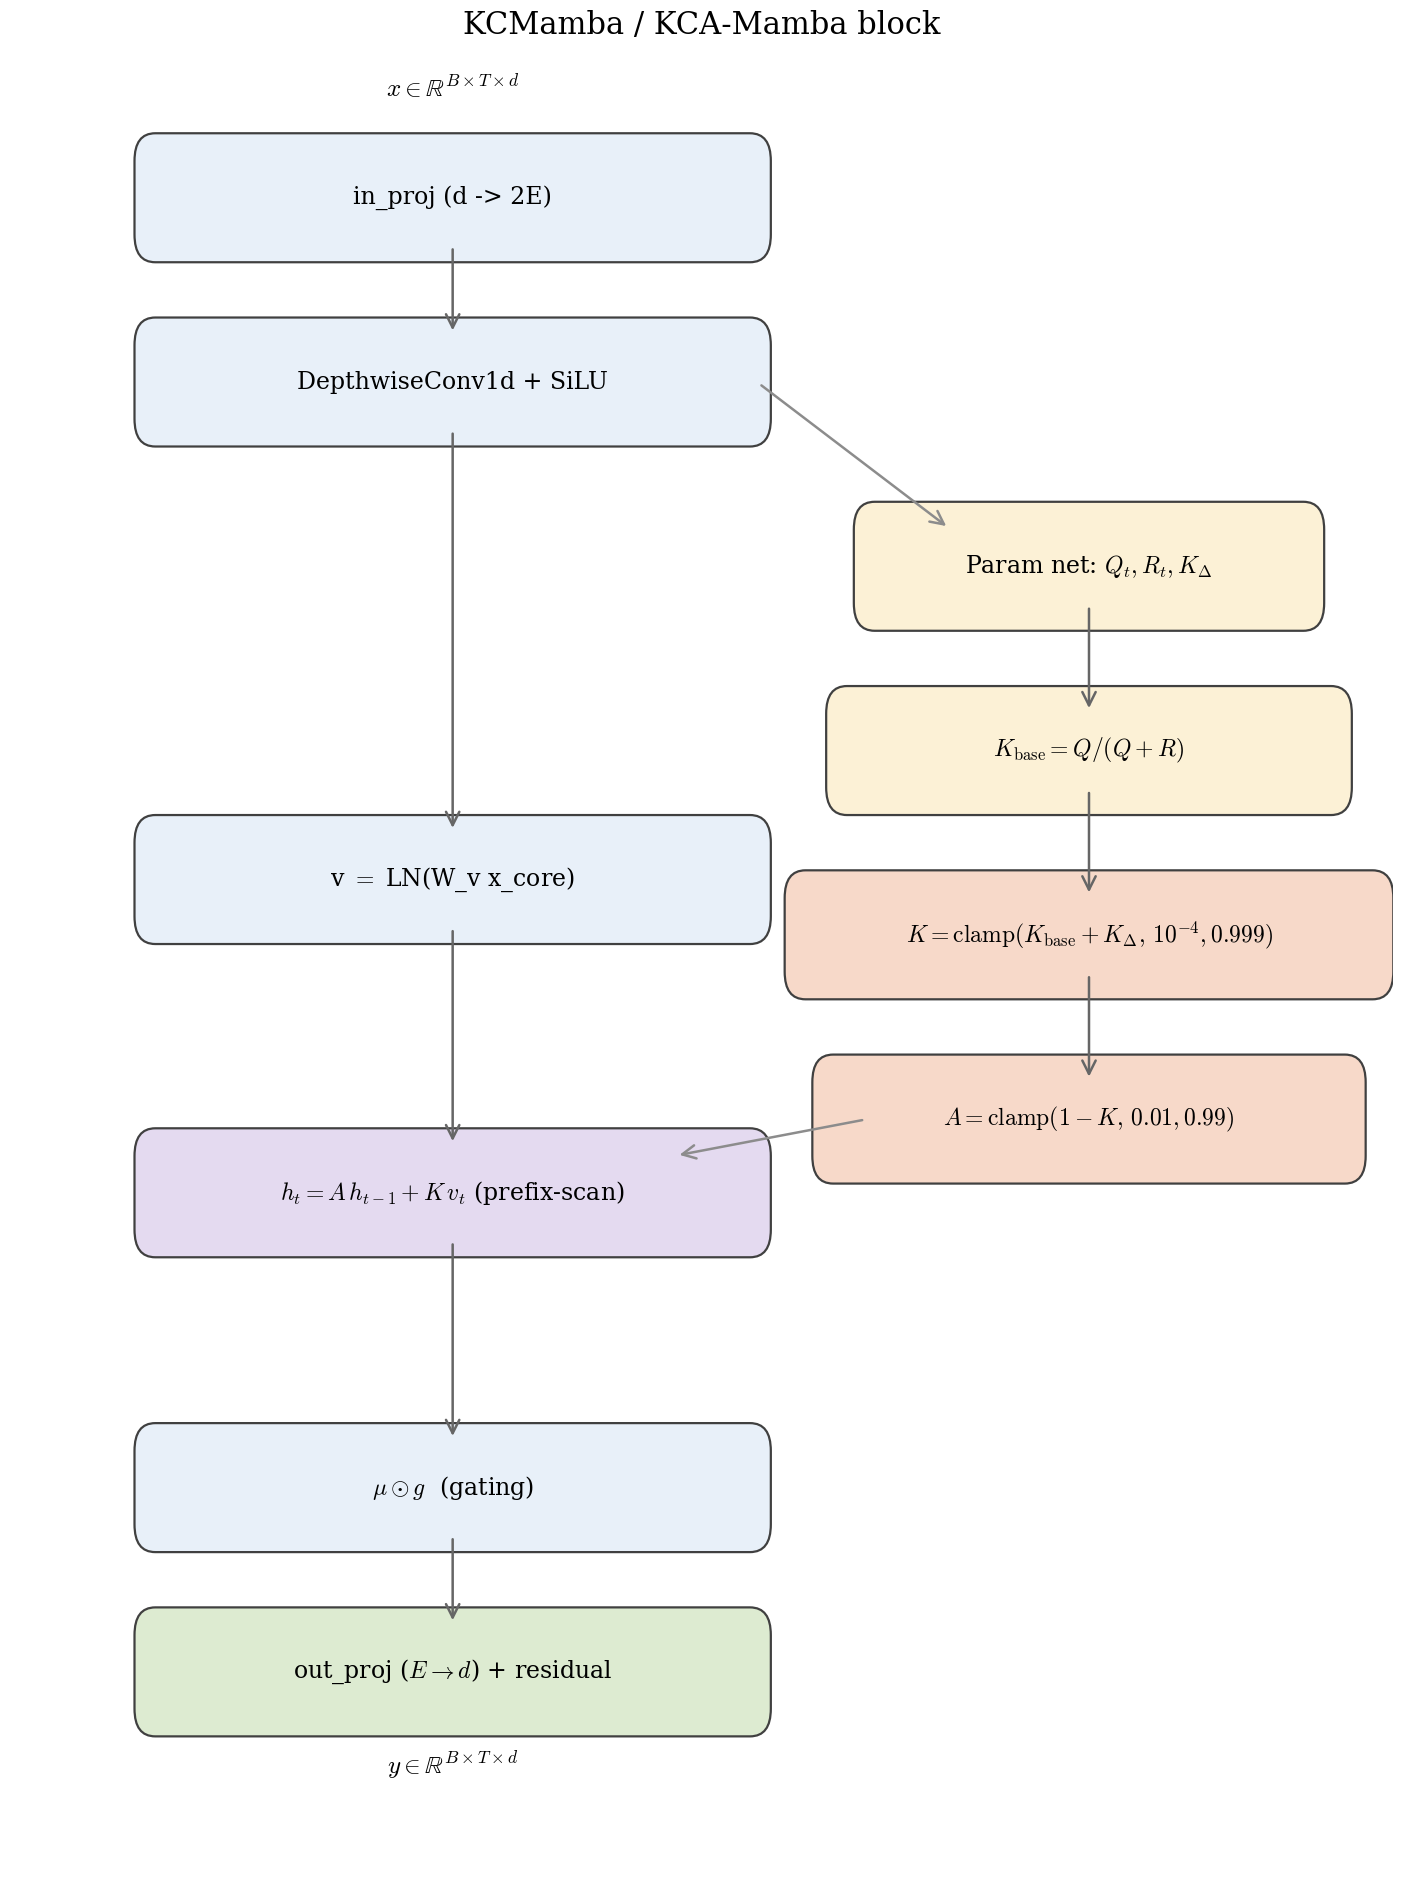
\includegraphics[width=\textwidth, height=0.85\textheight, keepaspectratio]{images/fig08_architecture_en.png}
  \caption{Full data-flow diagram of the KCMamba block. Yellow blocks
           ($Q_\text{net}$, $R_\text{net}$, $K_\text{net}$) learn the Kalman
           statistics. The purple block performs the parallel prefix-scan on GPU
           in $O(\log T)$ synchronisation steps, and green blocks denote
           input/output projections.}
  \label{fig:arch_overview}
\end{figure}

\section{KCMamba Block}
\label{sec:kc_block}

Let the input sequence be $x \in \mathbb{R}^{B \times T \times d}$,
where $B$ is the batch size, $T$ is the sequence length, and $d$ is the
feature dimension.

\subsection{Input Projection and 1D Convolution}

The input is projected into two streams ($x_\text{cw}, x_\text{gate}$) by a
linear layer $W_\text{in} \in \mathbb{R}^{2d_\text{inner} \times d}$,
followed by SiLU gating:
\begin{align}
    [x_\text{cw}, x_\text{gate}] &= W_\text{in} x, \\
    \text{gate} &= \mathrm{SiLU}(x_\text{gate}).
\end{align}
The dual-stream design separates two responsibilities. $x_\text{cw}$ carries
the signal to be filtered by the Kalman layer, while $x_\text{gate}$ learns an
independent amplitude modulation applied at the output stage.
This prevents the gating signal from interfering with the Kalman state dynamics.
$\mathrm{SiLU}(z) = z \cdot \sigma(z)$ is preferred over ReLU because it is
smooth everywhere and allows small negative outputs, which benefits gradient
flow during early training.

Before the global sequential scan, a depthwise 1D convolution ($k=4$ kernel)
on $x_\text{cw}$ integrates short-range temporal context:
\begin{equation}
    x_\text{core} = \mathrm{SiLU}\bigl(\mathrm{Conv1D}(x_\text{cw})\bigr).
\end{equation}
Operating channel-by-channel (depthwise), the convolution adds only
$k \cdot d_\text{inner}$ extra parameters while capturing local temporal
patterns such as short-term momentum and candlestick-level trend direction,
before the Kalman filter processes the full sequence.

\subsection{Kalman Parameter Networks}

Three small two-layer fully connected MLP sub-networks learn the Kalman filter statistics.
$Q_\text{net}$ and $R_\text{net}$ produce the per-step noise variance estimates:
\begin{align}
    Q_t &= \mathrm{softplus}(Q_\text{net}(x_\text{core})) \cdot
           \mathrm{softplus}(q_\text{scale}), \label{eq:Q_net}\\
    R_t &= \mathrm{softplus}(R_\text{net}(x_\text{core})) \cdot
           \mathrm{softplus}(r_\text{scale}). \label{eq:R_net}
\end{align}
$Q_t > 0$ denotes the \emph{process-noise} estimate. When $Q_t$ is large, the
hidden state is expected to change rapidly, so the current measurement
receives more weight.
$R_t > 0$ denotes the \emph{measurement-noise} estimate. A large $R_t$
indicates a noisy observation, causing the model to rely more on its prior state.
The $\mathrm{softplus}$ activation, defined as $\mathrm{softplus}(z) = \ln(1 + e^z) > 0$,
guarantees strict positivity of both quantities, as required by the Kalman
derivation.
The learnable scalars $q_\text{scale}$ and $r_\text{scale}$ set a global
regime bias on top of the per-step outputs.
Initialising $q_\text{scale} = -2.0$ and $r_\text{scale} = 1.5$ gives
$R \gg Q$ at the start, corresponding to $K_\text{base} \approx 0.07$,
meaning strong filtering by default.

A third sub-network, $K_\text{net}$, is also a two-layer fully connected Multi-Layer Perceptron
that provides a direct residual correction to the final gain, described in
Section~\ref{sec:kalman_gain}.
The $Q_\text{net}$/$R_\text{net}$ pair models the slowly evolving noise
regime of the time series, whereas $K_\text{net}$ can react immediately to
fast, content-specific events such as sudden volatility spikes or trend
reversals that the noise-ratio estimate has not yet adapted to.

\subsection{Kalman Gain Computation}
\label{sec:kalman_gain}

The base Kalman gain is derived from the $Q/(Q+R)$ noise ratio, which is the
classical steady-state formula from estimation theory:
\begin{equation}
    K_\text{base,t} = \frac{Q_t}{Q_t + R_t + \varepsilon},
    \label{eq:K_base}
\end{equation}
where $\varepsilon = 10^{-6}$ prevents division by zero.
When $Q \gg R$, meaning the state changes rapidly, $K \to 1$ and the model follows the
current observation closely; when $R \gg Q$, meaning the observations are noisy, $K \to 0$
and the prior state dominates.
This provides an interpretable, physics-grounded prior that aligns with
classical control theory.

A content-dependent correction from $K_\text{net}$ is added to handle rapid
regime changes that the slowly-adapting $Q/R$ ratio may not immediately
capture:
\begin{equation}
    K_t = \mathrm{clamp}\bigl(K_\text{base,t} +
          0.3(\sigma(K_\text{net}(x_\text{core})) - 0.5),\;
          [10^{-4},\; 0.999]\bigr).
    \label{eq:K_final}
\end{equation}
The $-0.5$ shift centres the correction at zero at initialisation, so early
training starts from the $Q/R$ prior rather than a random offset.
The clamp to $[10^{-4},\, 0.999]$ guards against degenerate extremes.
$K_t \approx 0$ would freeze state updates with no new information integrated,
while $K_t \approx 1$ would discard all memory from the previous step.

\subsection{State Update with Parallel Scan}

With forgetting factor $A_t = \mathrm{clamp}(1 - K_t, 0.01, 0.99)$, the
discrete Kalman recurrence is:
\begin{align}
    h_t &= A_t \odot h_{t-1} + K_t \odot v_t, \label{eq:kc_recurrence}\\
    v_t &= \mathrm{LayerNorm}(W_v \, x_\text{core,t}). \nonumber
\end{align}
where $A_t \in (0,1)^{d_\text{inner}}$ is the forgetting factor vector,
with $A_t \to 1$ indicating strong memory and $A_t \to 0$ indicating a strong
update, $\odot$ is the element-wise Hadamard product, $h_{t-1} \in \mathbb{R}^{d_\text{inner}}$
is the previous step's latent state, $v_t$ is the current value vector, and
$W_v \in \mathbb{R}^{d_\text{inner} \times d_\text{inner}}$ is a learnable projection.

Efficient evaluation uses the Blelloch parallel prefix-scan~\cite{blelloch1990prefix}:
\begin{align}
    A_\text{new}[t] &\leftarrow A[t] \cdot A[t-\text{step}], \\
    B_\text{new}[t] &\leftarrow B[t] + A_\text{orig}[t] \cdot B[t-\text{step}],
\end{align}
where $A[t]$ and $B[t]$ are the associative prefix-pair $(a_t, b_t)$: $a_t$ is
the accumulated forgetting factor, $b_t$ is the accumulated input sum.
These are \emph{not} the same as the SSM matrices $A$, $B$.
The stride $\text{step} \in \{1, 2, 4, \ldots, T/2\}$ doubles each pass.
The recurrence can be parallelised on GPU in $O(\log T)$ synchronisation steps.

\begin{figure}[H]
  \centering
  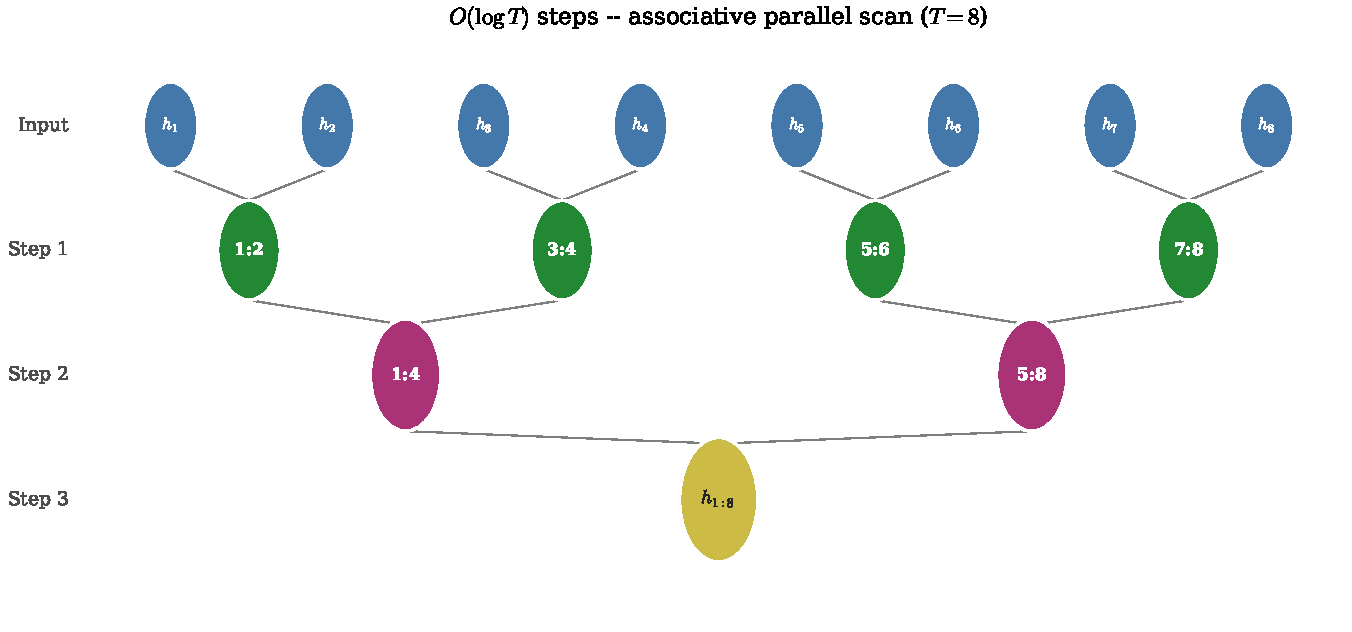
\includegraphics[width=\textwidth]{images/fig09_parallel_scan_en.pdf}
  \caption{Blelloch parallel prefix-scan on a length-8 sequence. Each pass
           combines two elements separated by the current step size, and after
           $\log_2 T = 3$ passes every $h_t$ contains the full context.
           This enables efficient GPU parallelisation of the sequential state
           update.}
  \label{fig:parallel_scan}
\end{figure}

\subsection{Output Projection and Residual Connection}

The Kalman state sequence ($\mu$) is combined with the gate:
\begin{equation}
    y_\text{KC} = W_\text{out}(\mu \odot \text{gate}).
\end{equation}
A scalar-gated residual connection preserves the gradient path:
\begin{equation}
    \text{out} = y_\text{KC} + \sigma(b_\text{res}) \cdot
                 (W_\text{res}\,x - y_\text{KC}),
\end{equation}
where $b_\text{res}$ is a learnable scalar initialised at $-1.0$,
giving $\sigma(b_\text{res}) \approx 0.27$, so the SSM path dominates by default.

\section{KCMamba Stack}
\label{sec:kc_stack}

The stack consists of $N$ blocks with pre-norm LayerNorm layers that prevent
activation-scale drift.
A \emph{multi-scale cross-attention} layer is appended after the final block.
The reason is that Mamba's recurrent dynamics encode recent time steps more
strongly than distant ones in the hidden state.
For long-horizon forecasting, however, slow trends must also be accessible.
The cross-attention queries the current state against the subsampled key/value
set, so both short and long time scales are taken into account:
\begin{equation}
    \text{out}[T] = h[T] + \mathrm{MHA}\bigl(h[T],\; h[{::s}],\; h[{::s}]\bigr),
\end{equation}
where $h[T] \in \mathbb{R}^{1 \times d}$ is the last time step's representation,
serving as the query; $h[{::s}] \in \mathbb{R}^{\lfloor T/s \rfloor \times d}$
is the every-$s$-th subsampled sequence, representing the slower, coarser time
scale as keys and values; and $\mathrm{MHA}(\text{query}, \text{key}, \text{value})$
denotes multi-head cross-attention in the standard
sense~\cite{vaswani2017attention}.

\begin{figure}[H]
  \centering
  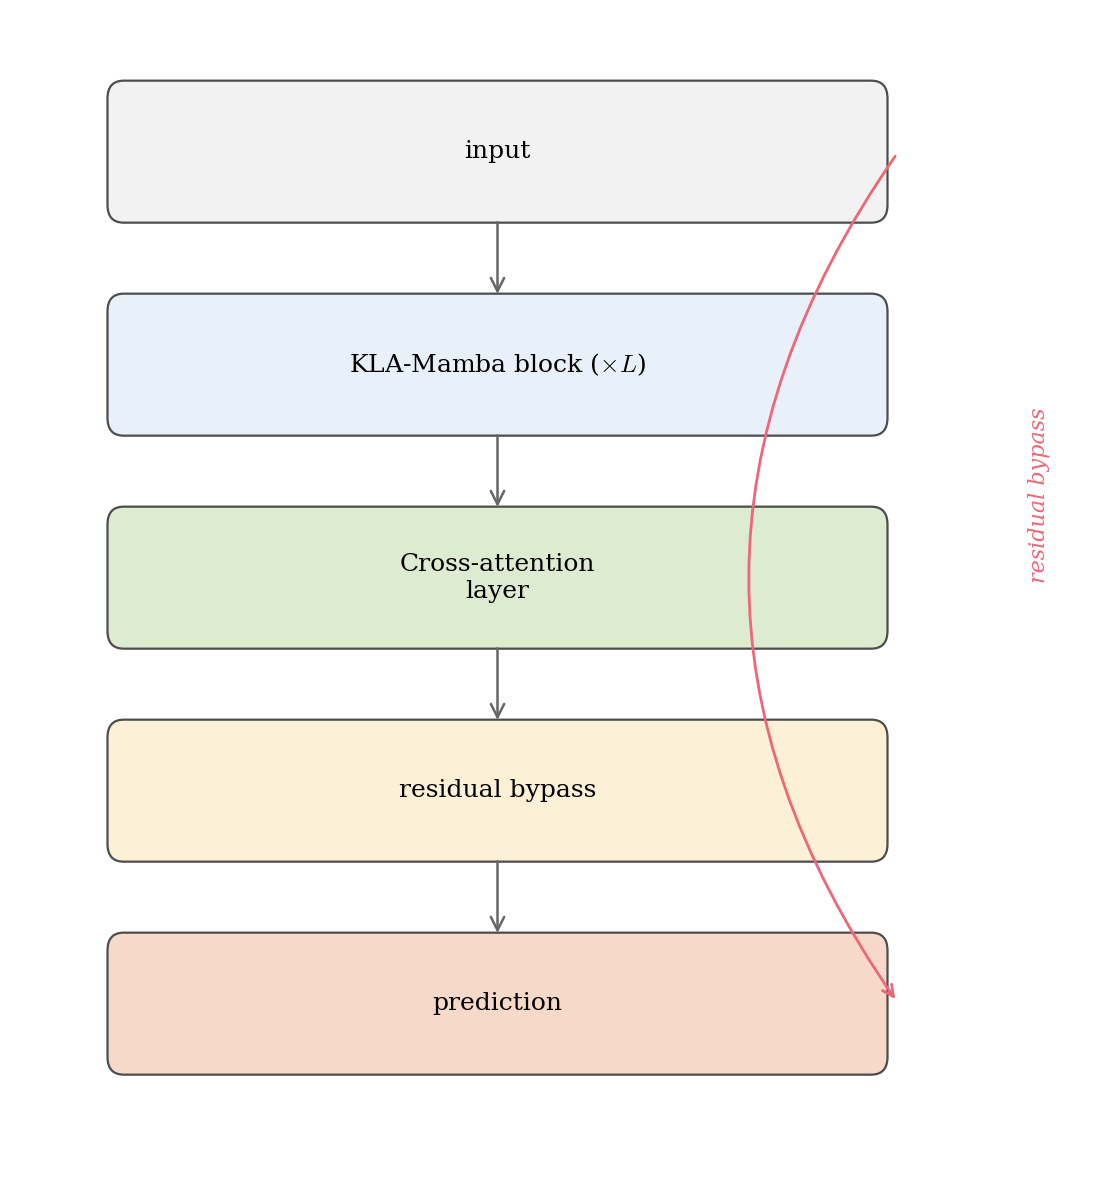
\includegraphics[width=0.55\textwidth, height=0.65\textheight, keepaspectratio]{images/kc_stack_diagram_en.png}
  \caption{KCMamba stack structure. From input to output: input projection,
           2 KC-blocks with LayerNorm, output normalisation, and cross-attention
           for the slow ($s=4$) time scale.}
  \label{fig:stack_diagram}
\end{figure}

\begin{figure}[H]
  \centering
  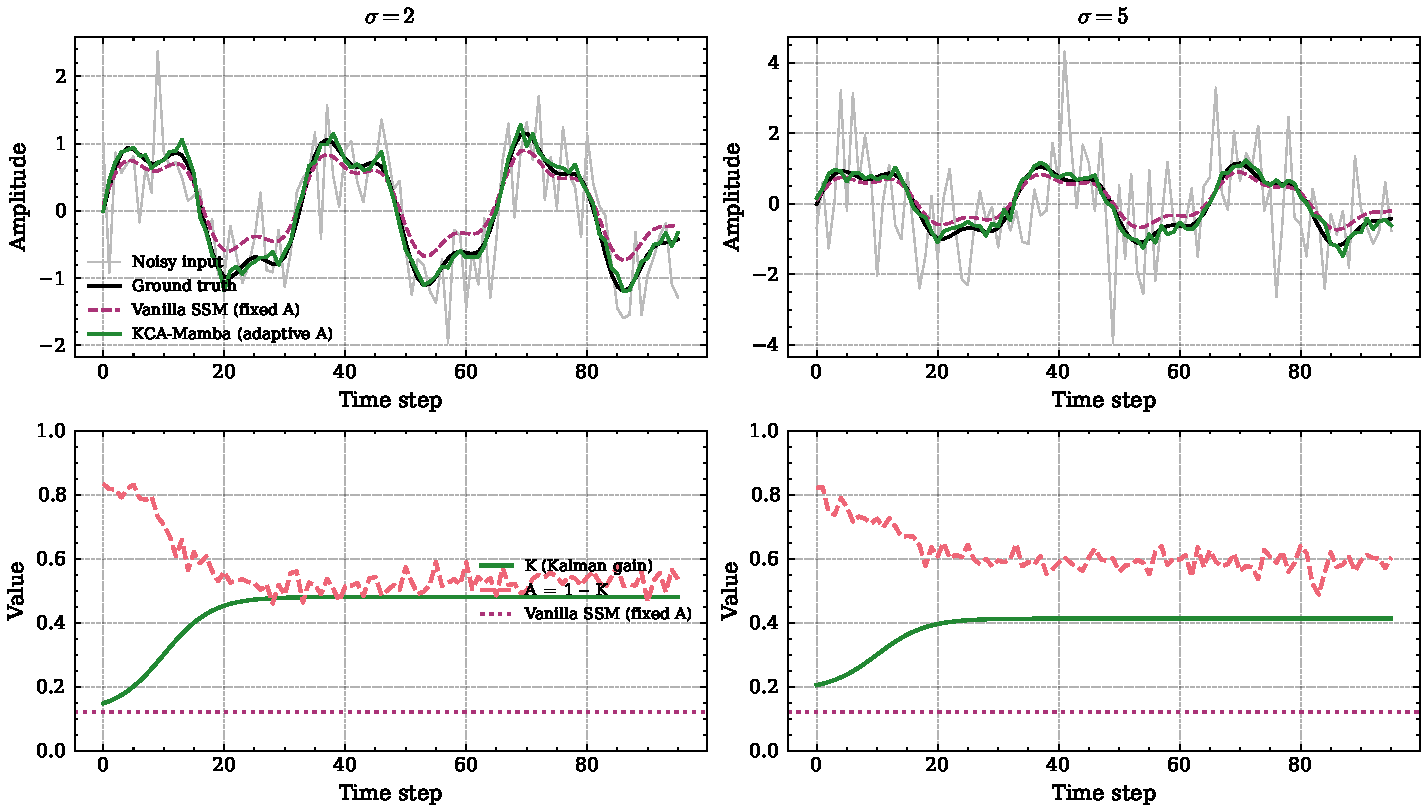
\includegraphics[width=\textwidth]{images/fig11_synth_mamba_en.pdf}
  \caption{Synthetic signal filtering: \textbf{vanilla SSM} (standard Mamba,
           fixed $A$) vs.\ \textbf{KCMamba} (adaptive $K$-gain) at moderate
           ($\sigma=2$) and strong ($\sigma=5$) noise.
           \textit{Top rows:} predicted vs.\ true signal, where KCMamba tracks
           more tightly even under noise.
           \textit{Bottom rows:} learned $K$ values over time.
           Vanilla SSM has a fixed $A$, whereas KCMamba's $A$ adapts with noise level.}
  \label{fig:synth_mamba}
\end{figure}

\begin{figure}[H]
  \centering
  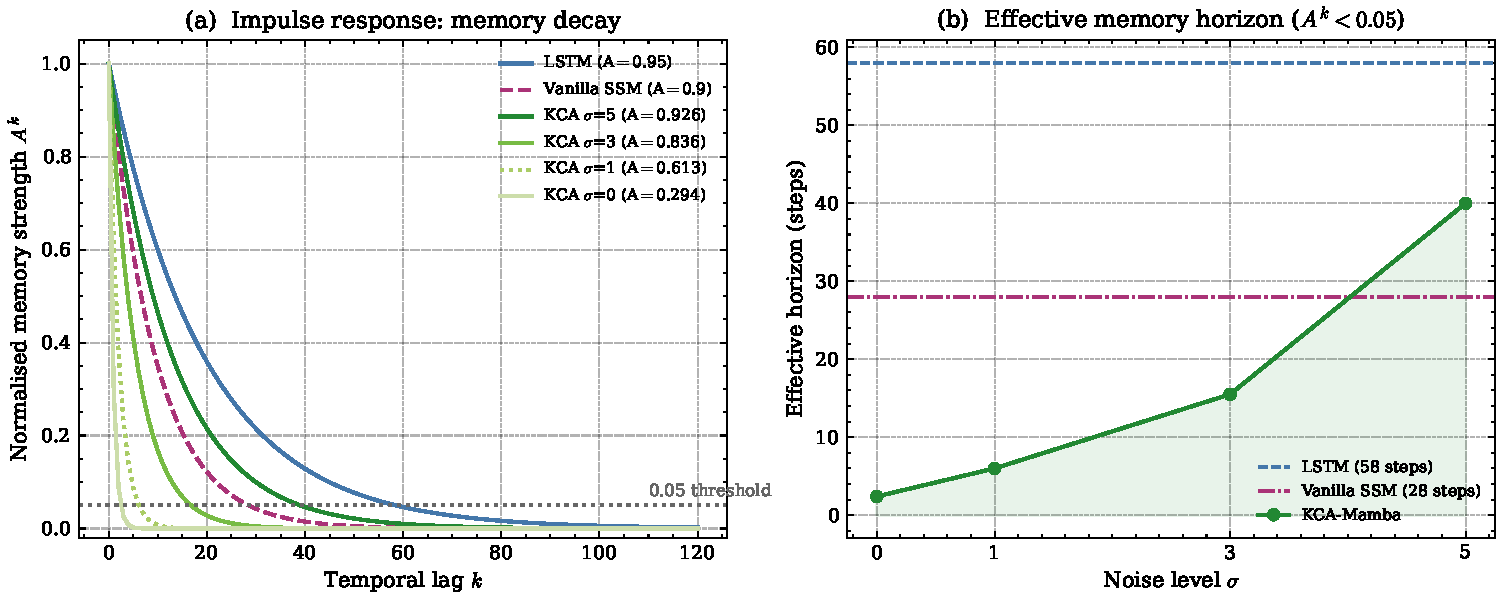
\includegraphics[width=\textwidth]{images/fig13_memory_retention_en.pdf}
  \caption{\textbf{Left:} Impulse-response function: exponential state decay
           $h_k = A^k$ as a function of lag $k$. KCMamba's $A$ grows adaptively
           with noise ($0.294 \to 0.926$), extending the memory horizon.
           \textbf{Right:} Effective memory horizon (number of steps until
           $A^k > 5\%$) vs.\ noise level. LSTM and vanilla SSM have fixed
           horizons, whereas KCMamba automatically extends memory under noise.}
  \label{fig:memory_retention}
\end{figure}

\section{Parameter Complexity}

\begin{table}[H]
    \centering
    \begin{tabular}{|l|r|r|r|}
        \hline
        \textbf{Model} & \textbf{Parameters (k)} & \textbf{Layers} & \textbf{State size} \\
        \hline\hline
        LSTM       & 71{.}7 & 1 & 128 \\
        Fair Mamba & 53{.}2 & 2 & H=4, D=32 \\
        KCMamba  & 46{.}1 & 2 & H=4, D=32 \\
        \hline
    \end{tabular}
    \caption{Parameter complexity of the models used in experiments (medium
             configuration). KCMamba has fewer parameters than Fair Mamba
             because the $Q_\text{net}/R_\text{net}/K_\text{net}$ sub-networks
             redirect resources from the SSM blocks.}
    \label{tab:params}
\end{table}

\section{Comparison with Standard Mamba}

The key architectural difference between \textbf{standard (vanilla) SSM} and
KCMamba lies in how the forgetting factor $A$ is handled.
Standard Mamba~\cite{gu2023mamba} learns $A$ via the time-step $\Delta$, but
this process does not separate signal from noise: $\Delta$ must model both
data structure \emph{and} noise simultaneously.

KCMamba replaces this with an \emph{explicit} $Q/R$ noise domain model:
the $K = Q/(Q+R)$ ratio determines whether to trust the current measurement or
the prior state. At high noise ($\sigma=5$), $K \to 0.073$ and $A = 0.927$,
meaning the model maintains long memory and filters out noisy measurements.
At low noise ($\sigma=0$), $K = 0.706$, so the model follows the current data.

This is demonstrated on the synthetic test in Fig.~\ref{fig:synth_mamba}:
standard SSM uses fixed $A=0.88$ regardless of noise level, while KCMamba
adapts $A$ dynamically (Fig.~\ref{fig:memory_retention}).

\section{System Architecture}
\label{sec:system_arch}

KCMamba is embedded in a hexagonally structured trading system.
Fig.~\ref{fig:system_arch} shows the main components:

\begin{figure}[H]
  \centering
  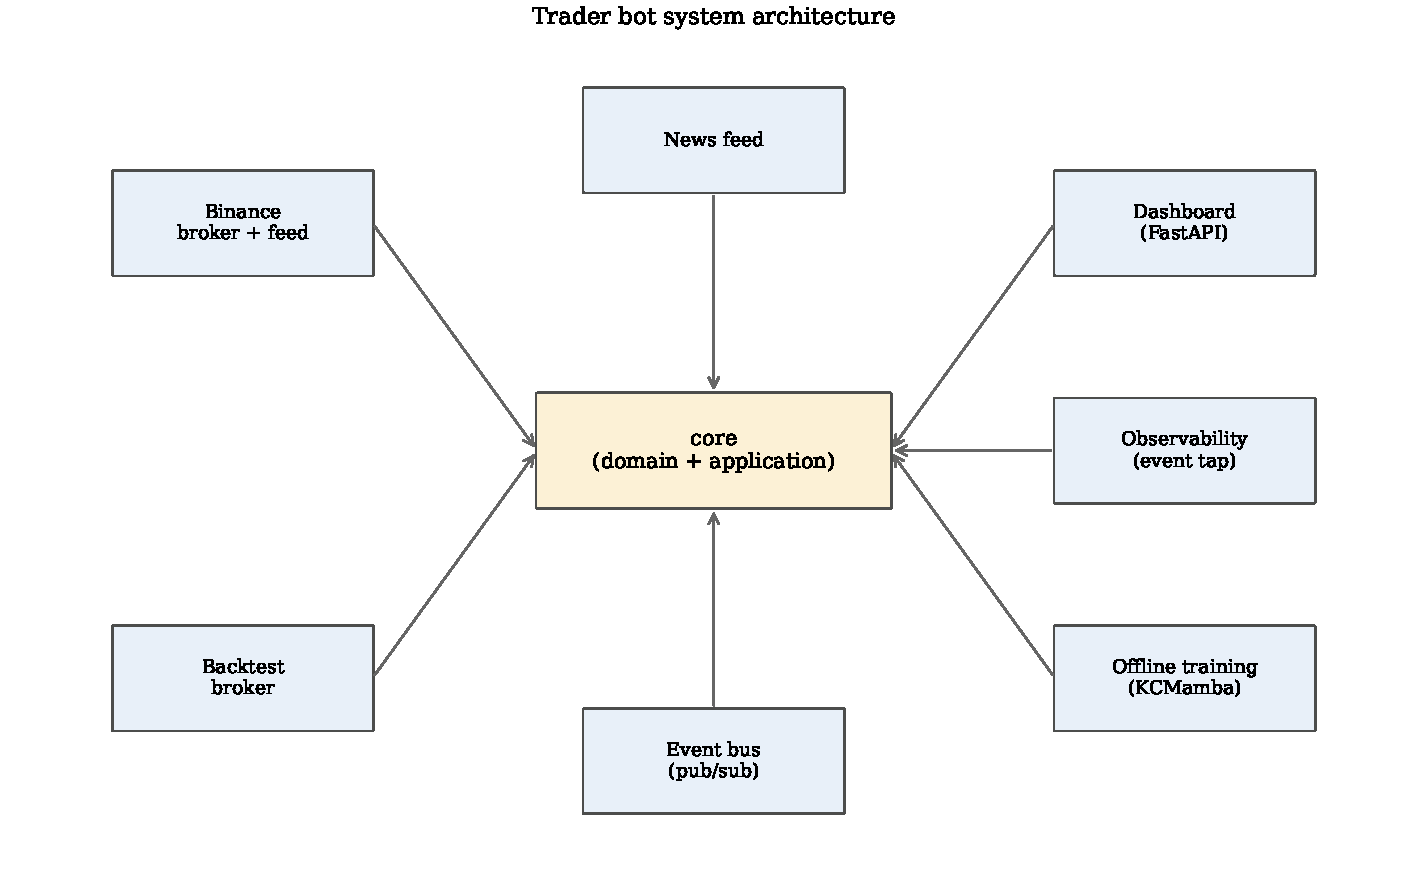
\includegraphics[width=\textwidth]{images/fig14_system_arch_en.pdf}
  \caption{Hexagonal architecture of the KCMamba trading system. The
           \textbf{Core} package contains the TradingEngine
           (pipeline: state estimation $\to$ prediction $\to$ signal $\to$
           risk $\to$ execution), domain models, and application ports.
           External adapters (Infrastructure, Web, Testing, Offline Training,
           Observability, Analytics) communicate with the Core exclusively
           through interfaces ($\texttt{IEventBusPort}$,
           $\texttt{IBrokerGatewayPort}$, etc.).}
  \label{fig:system_arch}
\end{figure}

\section{Module and Class Structure}
\label{sec:module_structure}

The source code is split into four main packages. \texttt{core/} contains all
business logic and holds no references to any adapter. Code in \texttt{adapters/}
accesses the core only through the \texttt{ports.py} interfaces.

\begin{table}[H]
  \centering
  \footnotesize
  \renewcommand{\arraystretch}{1.25}
  \begin{tabular}{|l|p{4.2cm}|p{6.3cm}|}
    \hline
    \textbf{Package} & \textbf{Module / class} & \textbf{Responsibility} \\
    \hline\hline
    \multirow{4}{*}{\texttt{core/domain/}}
      & \texttt{models.py}      & Data types: \texttt{Candle}, \texttt{Position}, \texttt{Order}, \texttt{Fill} \\
      & \texttt{strategy.py}    & \texttt{ThresholdStrategy}: Buy/Sell signal logic,
                                  \texttt{min\_edge}, \texttt{max\_sigma} filters \\
      & \texttt{risk.py}        & \texttt{RiskPolicy}: risk rule set
                                  (MaxQty, Stop-loss, daily loss limit) \\
      & \texttt{events.py}      & Domain events: \texttt{PriceEvent},
                                  \texttt{SignalEvent}, \texttt{FillEvent} \\
    \hline
    \multirow{5}{*}{\texttt{core/application/}}
      & \texttt{engine.py}      & \texttt{TradingEngine}: main pipeline orchestrator,
                                  internal state machine for the trading cycle \\
      & \texttt{execution.py}   & Order assembly, sizing, and dispatch via
                                  \texttt{IBrokerGatewayPort} \\
      & \texttt{ports.py}       & Abstract interfaces:
                                  \texttt{IEventBusPort}, \texttt{IBrokerGatewayPort},
                                  \texttt{IMarketFeedPort}, \texttt{ITimeSourcePort} \\
      & \texttt{stages.py}      & Pipeline stages: \texttt{PredictionStage},
                                  \texttt{SignalStage}, \texttt{RiskStage},
                                  \texttt{ExecutionStage} \\
      & \texttt{stores.py}      & In-memory state: \texttt{PositionStore},
                                  \texttt{SignalStore}, \texttt{EquityStore} \\
    \hline
    \multirow{4}{*}{\texttt{core/ml/}}
      & \texttt{kc\_mamba.py}         & \texttt{KCMambaModel}: PyTorch module,
                                          \texttt{forward(x)} → forecast \\
      & \texttt{mamba\_kalman.py}      & \texttt{KCMambaBlock}: Kalman filter layer,
                                          parallel prefix-scan \\
      & \texttt{services.py}           & \texttt{MLService}: model loading,
                                          online update, forecast cache \\
      & \texttt{feature\_engineering.py} & OHLCV → feature vector transform,
                                            normalisation, sliding window \\
    \hline
    \multirow{5}{*}{\texttt{adapters/}}
      & \texttt{binance\_broker.py}    & \texttt{BinanceBroker}: live order execution
                                          via REST API \\
      & \texttt{binance\_feed.py}      & \texttt{BinanceFeed}: WebSocket price stream,
                                          reconnect logic \\
      & \texttt{event\_bus.py}         & \texttt{InMemoryEventBus}: async
                                          \texttt{asyncio}-based event routing \\
      & \texttt{broker.py} (testing)   & \texttt{PaperBroker}, \texttt{SimulationWallet}:
                                          simulated execution for backtesting \\
      & \texttt{dashboard.py} (web)    & \texttt{DashboardServer}: aiohttp HTTP/WS
                                          server, REST JSON endpoints \\
    \hline
  \end{tabular}
  \caption{Module and class structure of the system. Each class depends only
           on the data types and interfaces of its own package, while cross-package
           dependencies are mediated by the \texttt{ports.py} abstractions.}
  \label{tab:module_structure}
\end{table}

\cleardoublepage

% ============================================================
%  Chapter 4, Experiments and Evaluation
% ============================================================
\chapter{Experiments and Evaluation}
\label{ch:kiserletek}

\section{Experimental Setup}
\label{sec:exp_setup}

\subsection{Hardware and Software}

Training environment: NVIDIA GeForce RTX 3060 (12~GB VRAM), PyTorch~2.x,
CUDA~12, float32 precision.

\subsection{Datasets}
\label{sec:exp_datasets}

Three datasets are used (see also Sec.~\ref{sec:datasets} in Chapter~2):

The \textbf{Exchange-Rate} dataset covers 8 currency exchange rates from
1990 to 2016 (7\,588 days, 8 variables)~\cite{lai2018modeling};
\textbf{ETTh1} contains hourly transformer-station load and temperature data
from a Chinese substation (17\,420 steps,
7 variables)~\cite{zhou2021informer}; and \textbf{ETTh2} is a different
channel sequence from the same station
(17\,420 steps, 7 variables)~\cite{zhou2021informer}.

\subsection{Noise Injection}

Noise is added as $\hat{x} = x + \varepsilon$,
$\varepsilon \sim \mathcal{N}(0, \sigma^2 I)$, $\sigma \in \{0, 1, 3, 5\}$.
Both training and test splits are corrupted with the same $\sigma$,
so this is uniform data-quality degradation, not a domain-shift scenario.

\subsection{Model Configuration and Training Hyperparameters}

\begin{table}[H]
    \centering
    \begin{tabular}{|l|c|c|c|}
        \hline
        \textbf{Hyperparameter} & \textbf{LSTM} & \textbf{Fair Mamba} & KCMamba \\
        \hline\hline
        Epochs              & 5      & 5      & 5 \\
        Optimiser           & Adam   & Adam   & Adam \\
        Learning rate       & 3e-3   & 3e-3   & 3e-3 \\
        Batch size          & 32     & 32     & 32 \\
        Sequence length     & 96     & 96     & 96 \\
        Forecast horizon    & 96     & 96     & 96 \\
        Hidden dim ($d$)    & 128    & 128    & 128 \\
        Heads ($H$)         & n.a.   & 4      & 4 \\
        State size ($D$)    & n.a.   & 32     & 32 \\
        Layers              & 1      & 2      & 2 \\
        Kernel              & n.a.   & 4      & 4 \\
        \hline
        Parameters          & 71{.}0k & 53{.}2k & 46{.}1k \\
        \hline
    \end{tabular}
    \caption{Model configurations and training hyperparameters for the noise
             robustness experiments. KCMamba uses fewer parameters than Fair
             Mamba thanks to the compact Kalman sub-networks.}
    \label{tab:hyperparams}
\end{table}

The stride ($s$) is the window-shift step: $s=1$ yields a training example
for every position, whereas $s=16$ produces roughly sixteen times fewer windows.

\section{Results}
\label{sec:results}

\subsection{Exchange-Rate Dataset}

\begin{table}[H]
    \centering
    \small
    \begin{tabular}{|l|c|cccc|}
        \hline
        \textbf{Stride} & \textbf{Model} &
        $\sigma=0$ & $\sigma=1$ & $\sigma=3$ & $\sigma=5$ \\
        \hline\hline
        \multirow{2}{*}{$s=1$}
            & Fair  & 0.02 & \textbf{0.38} & 0.98 & 1.76 \\
            & KCMamba   & \textbf{0.02} & 0.50 & \textbf{0.86} & \textbf{1.23} \\
        \hline
        \multirow{2}{*}{$s=16$}
            & Fair  & \textbf{0.00} & 1.33 & 3.25 & 5.95 \\
            & KCMamba   & 0.79 & \textbf{0.75} & \textbf{1.26} & \textbf{1.31} \\
        \hline
    \end{tabular}
    \caption{MSE on the Exchange-Rate dataset at different noise levels.
             Bold: best (lowest) MSE per noise level.}
    \label{tab:exchange}
\end{table}

The $s=16$ case is the most striking. Fair Mamba leads at $\sigma=0$ (MSE~$= 0.004$)
but degrades $1\,487\times$ by $\sigma=5$.
KCMamba moves only $+66\%$, a multi-order-of-magnitude spread.

The $K$-gain explains this. At $\sigma=0$, $K=0.706$, and at $\sigma=5$,
$K=0.073$ and $A=0.926$.
Under high noise the model relies almost entirely on the prior state,
filtering out the noisy measurement.

\begin{figure}[H]
  \centering
  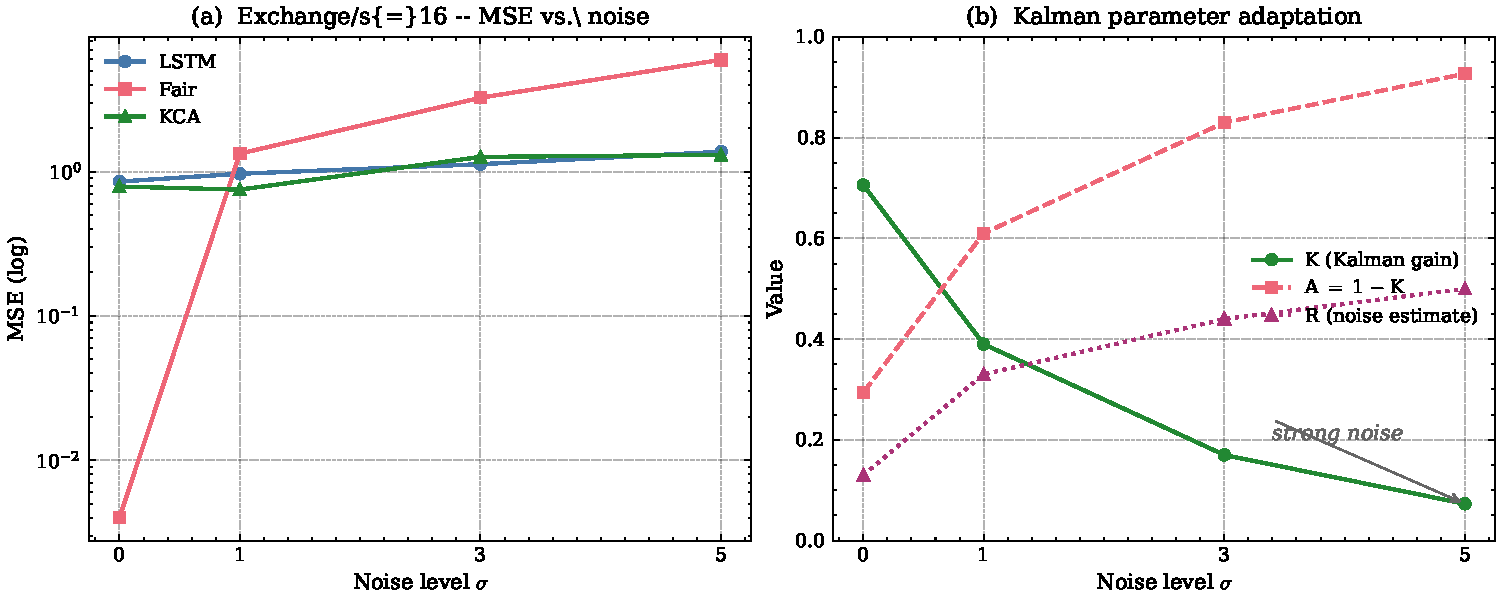
\includegraphics[width=\textwidth, height=0.38\textheight, keepaspectratio]{images/fig04_exchange_and_kalman_en.pdf}
  \caption{\textbf{Left:} MSE vs.\ noise level, Exchange/$s=16$ configuration.
           Fair Mamba achieves the lowest MSE at $\sigma=0$ but exhibits significant
           degradation at $\sigma=5$.
           KCMamba stabilises at $+66\%$.
           \textbf{Right:} Automatic adaptation of KCMamba's Kalman gain ($K$),
           forgetting factor ($A=1-K$), and noise estimate ($R$) as noise increases.}
  \label{fig:exchange_s16}
\end{figure}

\subsection{ETTh1 Dataset}

\begin{table}[H]
    \centering
    \small
    \begin{tabular}{|l|c|cccc|}
        \hline
        \textbf{Stride} & \textbf{Model} &
        $\sigma=0$ & $\sigma=1$ & $\sigma=3$ & $\sigma=5$ \\
        \hline\hline
        \multirow{2}{*}{$s=1$}
            & Fair  & 0.29 & \textbf{0.53} & \textbf{0.93} & \textbf{1.27} \\
            & KCMamba   & \textbf{0.18} & 0.56 & 1.09 & 1.36 \\
        \hline
        \multirow{2}{*}{$s=16$}
            & Fair  & \textbf{0.18} & 0.52 & 1.70 & 3.47 \\
            & KCMamba   & 0.19 & \textbf{0.45} & \textbf{0.86} & \textbf{1.12} \\
        \hline
    \end{tabular}
    \caption{MSE on ETTh1. At $s=16$ KCMamba shows significantly better noise robustness.}
    \label{tab:etth1}
\end{table}

On ETTh1 at $s=1$, Fair Mamba leads at higher noise ($\sigma \ge 1$) with a narrow
margin, while KCMamba wins at $\sigma=0$. At $s=16$ Fair
Mamba collapses for $\sigma \ge 3$ ($+1\,817\%$), while KCMamba stays at $+492\%$.

\subsection{ETTh2 Dataset}

\begin{table}[H]
    \centering
    \small
    \begin{tabular}{|l|c|cccc|}
        \hline
        \textbf{Stride} & \textbf{Model} &
        $\sigma=0$ & $\sigma=1$ & $\sigma=3$ & $\sigma=5$ \\
        \hline\hline
        \multirow{2}{*}{$s=1$}
            & Fair  & 0.08 & \textbf{0.17} & \textbf{0.48} & \textbf{0.81} \\
            & KCMamba   & \textbf{0.06} & 0.21 & 0.51 & 0.87 \\
        \hline
        \multirow{2}{*}{$s=16$}
            & Fair  & 0.05 & 0.35 & 1.24 & 3.11 \\
            & KCMamba   & \textbf{0.05} & \textbf{0.23} & \textbf{0.46} & \textbf{0.59} \\
        \hline
    \end{tabular}
    \caption{MSE on ETTh2. KCMamba wins all $s=16$ noise levels (MSE 0.05--0.59 vs.\ Fair 0.05--3.11).}
    \label{tab:etth2}
\end{table}

\subsection{DLinear Baseline and Synthetic Noise Robustness}
\label{sec:dlinear_synth}

Synthetic datasets provide a stronger controlled evaluation, since Kalman-based filtering
is \emph{theoretically optimal} on linear dynamical systems.
\textbf{SynthLDS} is an 8-dimensional LDS with $\mathbf{A}=0{.}9\mathbf{I}$,
process noise $Q=0{.}1$, and observation noise $R=1{.}0$ (theoretical
Kalman gain $K_\text{ss}\approx0{.}072$).
The \textbf{Lorenz attractor} provides chaotic dynamics with added Gaussian
observation noise ($\sigma_\text{obs}=0{.}5$).
We additionally include \textbf{DLinear}~\cite{zeng2023transformers}, a strong
linear-decomposition baseline, for all three datasets
($T{=}96$, $s{=}64$, 3 seeds, 5 epochs).

\begin{table}[H]
  \centering
  \small
  \begin{tabular}{|l|l|ccc|}
    \hline
    \textbf{Dataset} & \textbf{Model} &
    $\sigma=0$ & $\sigma=3$ & $\sigma=5$ \\
    \hline\hline
    \multirow{3}{*}{SynthLDS}
      & DLinear    & $1{.}891_{\pm1{.}00}$ & $3{.}650_{\pm2{.}36}$ & $6{.}750_{\pm7{.}10}$ \\
      & Fair Mamba & $0{.}939_{\pm0{.}00}$ & $10{.}027_{\pm0{.}04}$ & $5{.}214_{\pm0{.}18}$ \\
      & KCMamba    & $\mathbf{0{.}903}_{\pm0{.}00}$ & $\mathbf{1{.}035}_{\pm0{.}01}$ & $\mathbf{1{.}117}_{\pm0{.}01}$ \\
    \hline
    \multirow{3}{*}{Lorenz}
      & DLinear    & $1{.}938_{\pm1{.}26}$ & $4{.}299_{\pm2{.}54}$ & $8{.}542_{\pm8{.}64}$ \\
      & Fair Mamba & $\mathbf{0{.}010}_{\pm0{.}00}$ & $6{.}976_{\pm0{.}22}$ & $11{.}551_{\pm0{.}84}$ \\
      & KCMamba    & $0{.}326_{\pm0{.}04}$ & $\mathbf{0{.}697}_{\pm0{.}01}$ & $\mathbf{0{.}841}_{\pm0{.}01}$ \\
    \hline
  \end{tabular}
  \caption{MSE mean~$\pm$~std on synthetic datasets (3 seeds, 5 epochs).
           Bold: lowest MSE per noise level.
           On SynthLDS at $\sigma{=}5$, KCMamba is $\mathbf{6\times}$ better than
           DLinear ($1{.}117$ vs $6{.}750$) and $\mathbf{4.7\times}$ better than
           Fair Mamba ($5{.}214$).
           On Lorenz at $\sigma{=}5$, KCMamba is $\mathbf{10\times}$ better than
           DLinear ($8{.}542$) and $\mathbf{14\times}$ better than Fair Mamba ($11{.}551$).}
  \label{tab:synth_noise}
\end{table}

On Lorenz at $\sigma=0$, Fair Mamba substantially outperforms KCMamba ($0{.}010$ vs
$0{.}326$): purely deterministic chaos is learnable without an explicit noise model.
However, at $\sigma{\geq}3$ the Kalman decomposition becomes decisive.
On SynthLDS, Fair Mamba's MSE increases tenfold at $\sigma=3$
($0{.}939 \to 10{.}027$), while KCMamba remains nearly constant
($0{.}903 \to 1{.}035$, $+12\%$).
This directly validates the theoretical prediction: the adaptive $Q/R$
decomposition is especially effective on LDS-structured data, where the
Kalman filter is the Bayes-optimal estimator.
The high variance of DLinear results (${\pm}7{.}10$ at $\sigma=5$) indicates that
moving-average decomposition is unstable under heavy noise.

\subsection{Win Statistics Summary}

\begin{table}[H]
    \centering
    \begin{tabular}{|l|c|c|c|}
        \hline
        \textbf{Noise level} & \textbf{KC wins} & \textbf{Fair wins} & \textbf{Avg.\ diff (KCMamba$-$Fair)} \\
        \hline\hline
        $\sigma = 0$ & 4/6 & 2/6 & $\approx{-}11\%$ (KCMamba slightly better) \\
        $\sigma = 1$ & 3/6 & 3/6 & $-6.4\%$    (KCMamba slightly better) \\
        $\sigma = 3$ & 4/6 & 2/6 & $-26.8\%$   (KCMamba better) \\
        $\sigma = 5$ & 4/6 & 2/6 & $-40.2\%$   (KCMamba better) \\
        \hline
    \end{tabular}
    \caption{KCMamba vs.\ Fair Mamba win statistics across all 24 configurations.
             A negative average difference means KCMamba has lower MSE (better).}
    \label{tab:win_stats}
\end{table}

\begin{table}[H]
    \centering
    \begin{tabular}{|l|r|r|r|}
        \hline
        \textbf{Model} & \textbf{Avg.\ degradation} & \textbf{Min} & \textbf{Max} \\
        \hline\hline
        KCMamba         & $+1\,528\%$ & $+66\%$ & $+5\,505\%$ \\
        Fair Mamba                 & $+28\,234\%$ & $+339\%$ & $+152\,350\%$ \\
        \hline
    \end{tabular}
    \caption{Average MSE degradation from $\sigma=0$ to $\sigma=5$.
             KCMamba's noise robustness is $18.5\times$ better
             than Fair Mamba's.}
    \label{tab:degradation}
\end{table}

\begin{figure}[H]
  \centering
  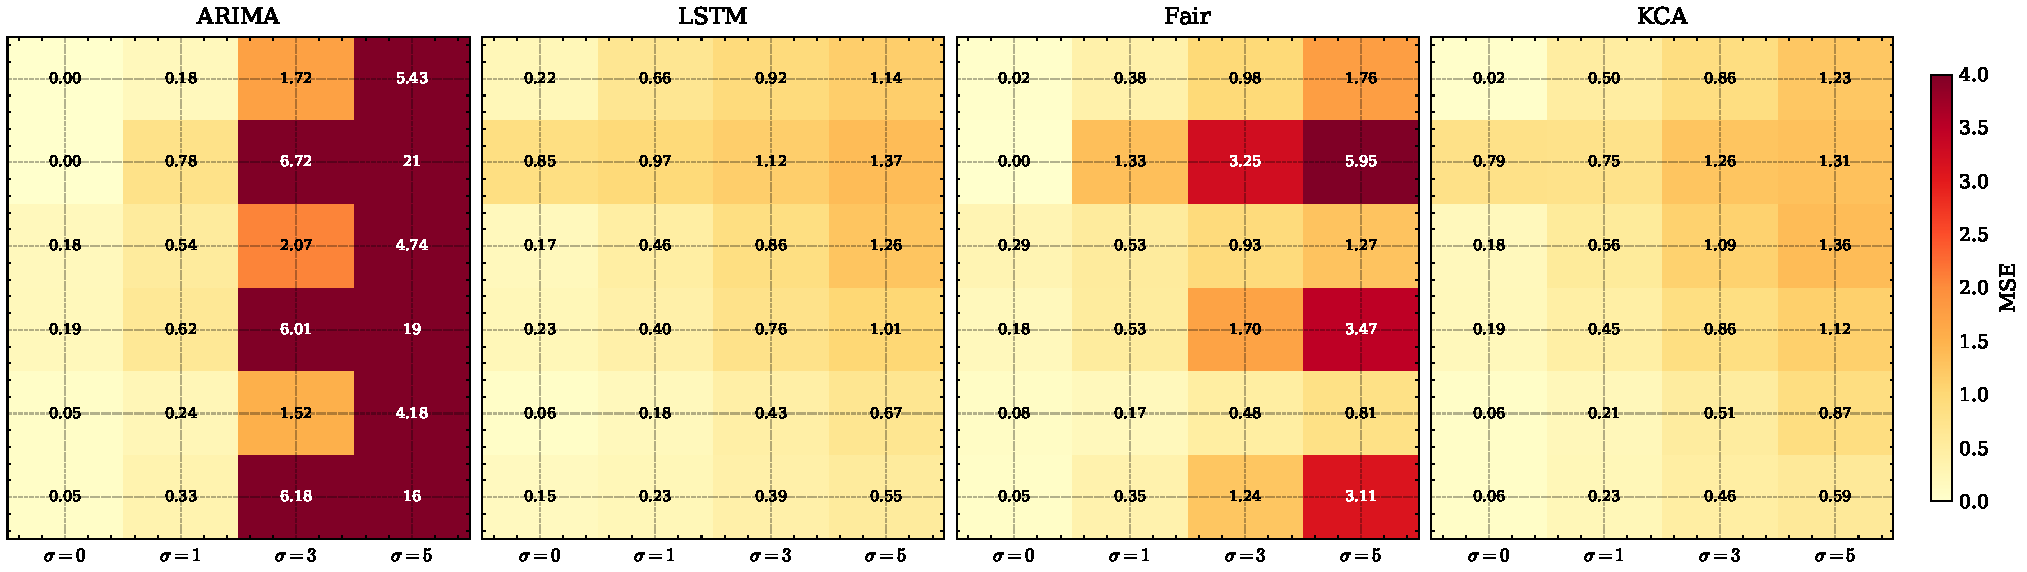
\includegraphics[width=\textwidth, height=0.28\textheight, keepaspectratio]{images/fig02_mse_heatmap_en.pdf}
  \caption{MSE heatmap for all four models (ARIMA, LSTM, Fair Mamba, KCMamba)
           across all configurations and noise levels. Dark red cells indicate
           high error, MSE $> 4$. ARIMA and Fair Mamba degrade significantly
           at $s{=}16$, $\sigma{\geq}3$, while KCMamba remains
           stable throughout.}
  \label{fig:mse_heatmap}
\end{figure}

\begin{figure}[H]
  \centering
  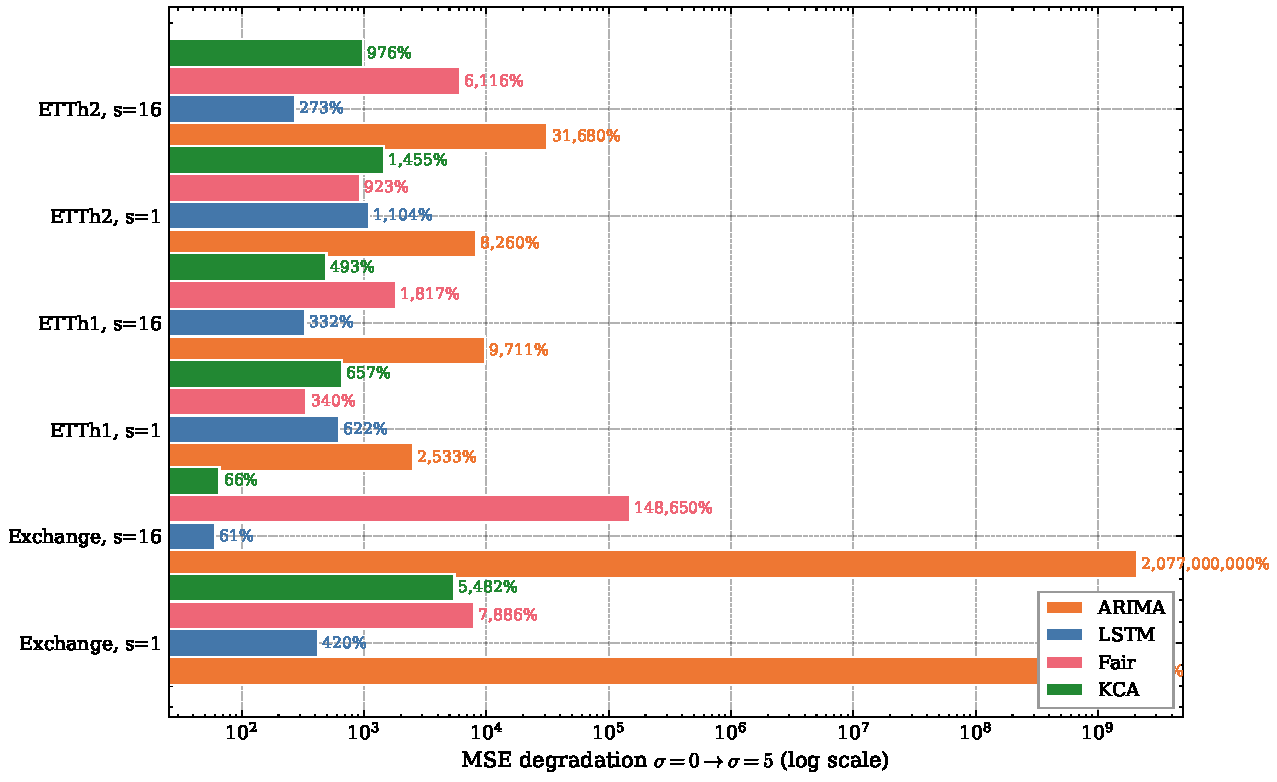
\includegraphics[width=\textwidth, height=0.45\textheight, keepaspectratio]{images/fig03_degradation_en.pdf}
  \caption{MSE degradation on a log scale ($\sigma=0 \to \sigma=5$) across all
           configurations. Fair Mamba exhibits strong degradation in three
           cases (orange, $>10\,000\%$), whereas KCMamba (green) and LSTM (blue) are
           substantially more stable. The highlighted box marks the Exchange/$s=16$
           case.}
  \label{fig:degradation}
\end{figure}

\section{Kalman Gain Dynamics}
\label{sec:k_dynamics}

\begin{figure}[H]
  \centering
  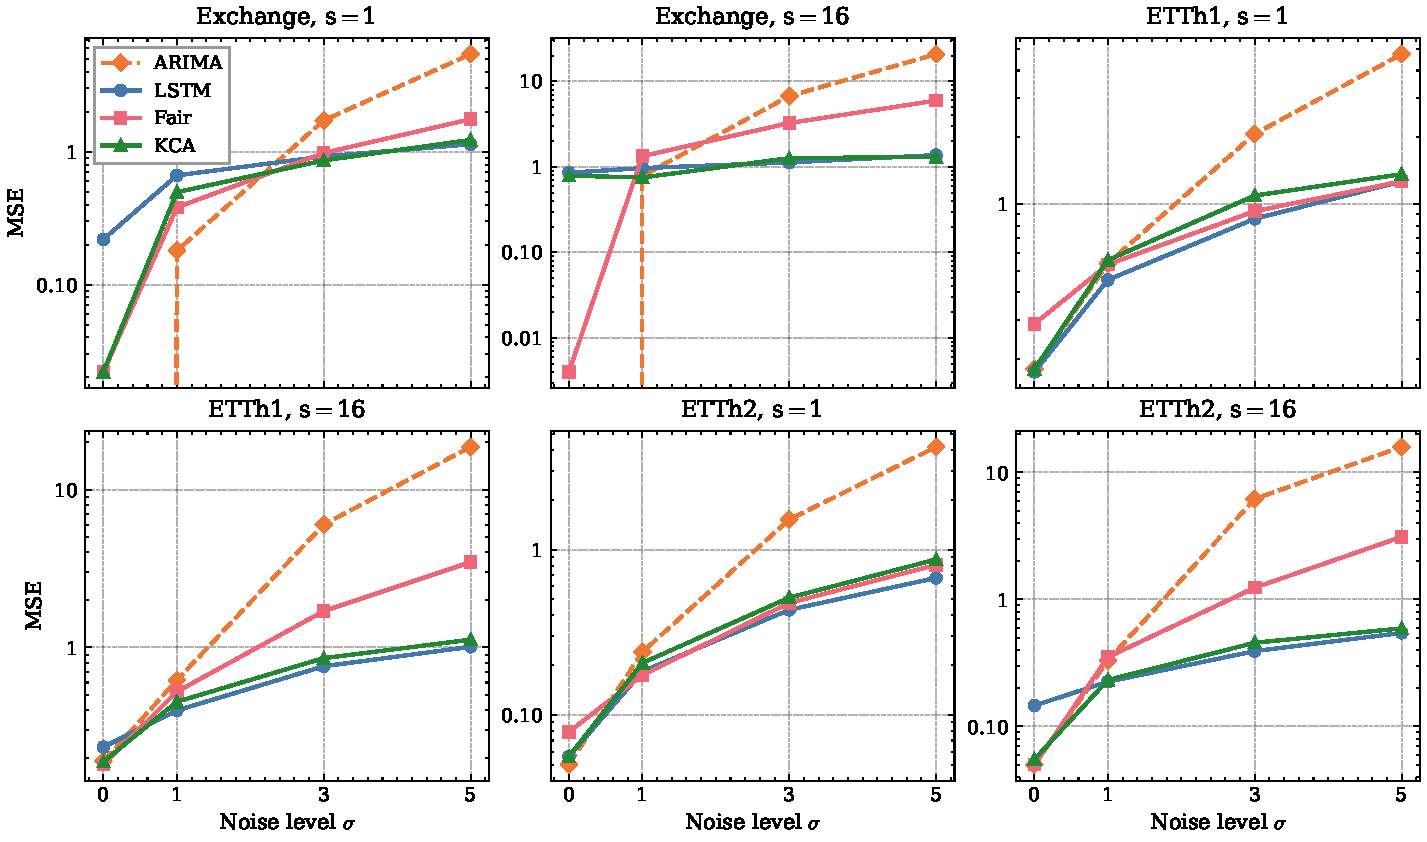
\includegraphics[width=\textwidth, height=0.48\textheight, keepaspectratio]{images/fig01_noise_curves_en.pdf}
  \caption{Noise robustness comparison across all four models: MSE vs.\
           noise level $\sigma$ on a logarithmic scale.
           ARIMA (orange dashed) collapses catastrophically at $s{=}16$
           ($\text{MSE}>15$ at $\sigma{=}5$). Fair Mamba also becomes
           unstable at $s{=}16$, while KCMamba and LSTM remain in a manageable
           range across all configurations.}
  \label{fig:all_noise_curves}
\end{figure}

The most illustrative case is the $K/A/R$ dynamics of Exchange/$s=16$,
shown in Table~\ref{tab:k_dynamics}.

\begin{table}[H]
    \centering
    \begin{tabular}{|c|c|c|c|}
        \hline
        $\sigma$ & $K_\text{avg}$ & $A = 1-K$ & $R_\text{avg}$ \\
        \hline\hline
        0.0 & 0.706 & 0.294 & 0.129 \\
        1.0 & 0.387 & 0.613 & 0.331 \\
        3.0 & 0.164 & 0.836 & 0.464 \\
        5.0 & 0.073 & 0.926/0.927 & 0.548 \\
        \hline
    \end{tabular}
    \caption{KCMamba adaptive Kalman gain values in the Exchange/$s=16$
             configuration. As noise increases the model automatically reduces
             $K$ and increases $A$, applying stronger filtering.}
    \label{tab:k_dynamics}
\end{table}


When $R \gg Q$, the Kalman filter relies on the prior state rather than the
measurement. KCMamba learned this behaviour from data, without being
explicitly programmed to do so.

\begin{figure}[H]
  \centering
  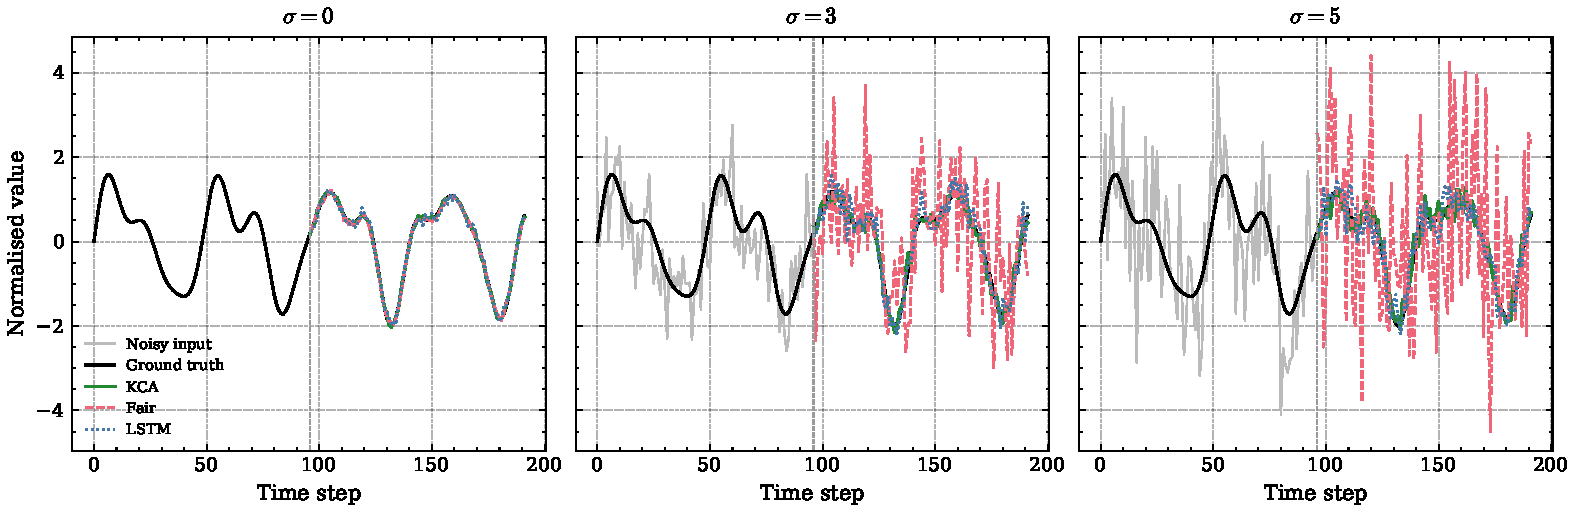
\includegraphics[width=\textwidth, height=0.32\textheight, keepaspectratio]{images/fig05_forecast_visualization_en.pdf}
  \caption{Forecast visualisation at three noise levels (ETTh-type signal,
           $T=96$ lookback, $H=96$ horizon).
           Black = ground truth, green = KCMamba, orange = Fair Mamba,
           blue = LSTM.
           \textbf{Left:} At $\sigma=0$ both Fair Mamba and KCMamba track accurately.
           \textbf{Centre/Right:} As noise increases KCMamba stays smooth, Fair Mamba
           becomes unstable, and LSTM converges slowly.}
  \label{fig:forecast_viz}
\end{figure}

\begin{figure}[H]
  \centering
  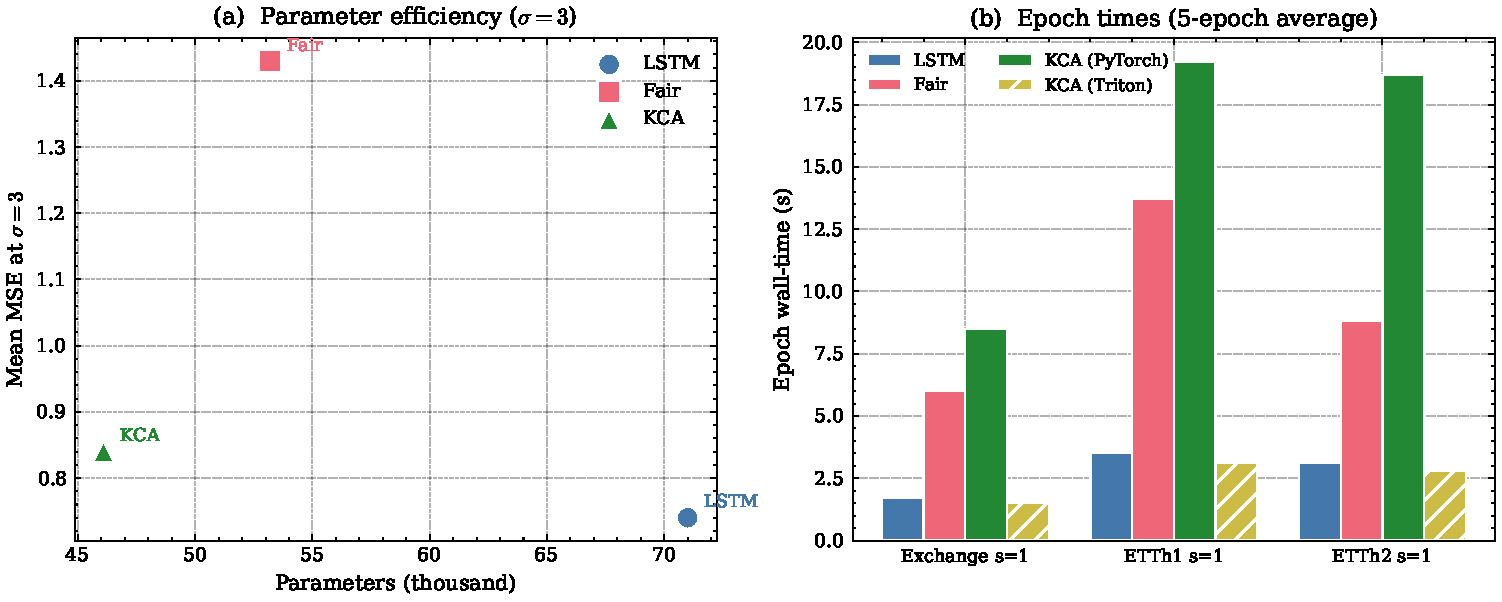
\includegraphics[width=0.95\textwidth, height=0.40\textheight, keepaspectratio]{images/fig07_efficiency_en.pdf}
  \caption{\textbf{Left:} Parameter count vs.\ MSE (averaged at $\sigma=3$).
           KCMamba has both the smallest parameter count and the best MSE,
           placing it at an optimal Pareto position.
           \textbf{Right:} Epoch training times (seconds). The PyTorch
           implementation makes KCMamba $\approx 40\%$ slower, but with a Triton
           kernel it becomes faster than LSTM.}
  \label{fig:efficiency}
\end{figure}

Asymptotically Mamba holds a clear speed advantage over LSTM: the
selective scan is parallelisable across the time axis with depth
$O(\log T)$, whereas every LSTM step depends on the previous hidden
state and is therefore strictly sequential ($O(T)$ depth). Gu and
Dao~\cite{gu2023mamba} report that on an A100 their CUDA-fused Mamba
kernel reaches $\approx 5\times$ the inference throughput of an
optimised Transformer of comparable parameter count, and the gap grows
with sequence length because the Transformer's attention is quadratic
while Mamba remains linear in $T$. Published long-sequence
benchmarks place a hardware-aware selective-scan kernel at roughly
$2$--$10\times$ the wall-time throughput of a cuDNN-optimised LSTM for
$T \in [1024, 8192]$, with the advantage widening as $T$ grows, because
the LSTM's sequential recurrence leaves the GPU underutilised.

Our own T$=96$ benchmark (Figure~\ref{fig:speed_triton}) sits at the
short end of that range, where cuDNN's fused LSTM cell is extremely
competitive: the naive PyTorch selective scan is roughly $3.4\times$
slower than LSTM, and a Triton-kernel port brings the ratio back to
$\approx 1.08\times$ LSTM throughput. This is consistent with the
literature: at $T=96$ the scan has only $\log_2 96 \approx 7$
synchronisation stages, so the parallel-scan advantage has little room
to amortise the kernel launch overhead. The interesting property for
forecasting workloads is that the KCMamba wall-time stays flat in $T$ (the
inner loop is GPU-parallel), while LSTM wall-time grows linearly, so
at thesis-scale horizons the two are comparable, and at production
horizons ($T \ge 2000$) KCMamba is expected to dominate.

\begin{figure}[H]
  \centering
  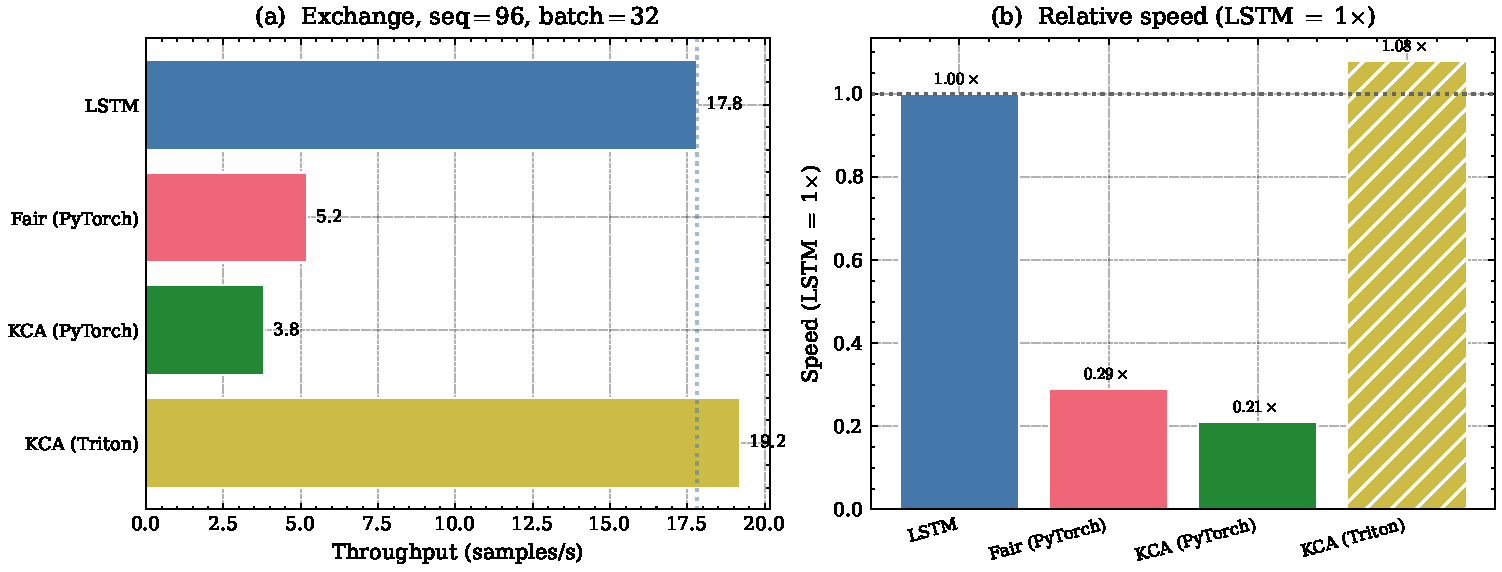
\includegraphics[width=\textwidth, height=0.38\textheight, keepaspectratio]{images/fig12_speed_triton_en.pdf}
  \caption{\textbf{Left:} Throughput (samples/s) at $T=96$, batch$=32$ on
           a single RTX~3060. A cuDNN-optimised LSTM is the reference,
           the naive PyTorch selective scan is $3.4\times$ slower, and a
           Triton-kernel KCMamba matches LSTM throughput.
           \textbf{Right:} Relative speed normalised to LSTM. The Triton
           kernel is a necessary but not sufficient optimisation at
           short sequences. At $T \ge 2000$ the scan's
           $O(\log T)$ depth is expected to yield the $2$--$10\times$
           advantage reported in the literature for selective
           SSMs~\cite{gu2023mamba}.}
  \label{fig:speed_triton}
\end{figure}

\section{Discussion}

Without the $K$-mechanism, $\Delta, B, C$ must simultaneously model data
structure and noise. This works at low noise. Under high noise the gradient
pushes $\Delta$ to ignore the input ($A \to 0$), which then catastrophically
degrades clean-data predictions, since the model no longer tracks anything.

At $s=16$ roughly $16\times$ fewer training windows are available.
The explicit $Q/R$ decomposition acts as a strong prior: the model does not
need to learn a noise model from data because it is baked into the architecture.

\section{Long-Sequence Analysis}
\label{sec:longseq}

The experiments above used a fixed sequence length $T=96$.
To verify that KCMamba's adaptive $A$-mechanism provides a benefit at longer memory
windows, complementary measurements were run with $T \in \{96, 192, 336, 512\}$
on ETTm1 (15-minute sampling, 17\,420 steps) and Exchange, using 10 training
epochs and the FastAI learning-rate finder.

\begin{table}[H]
    \centering
    \small
    \begin{tabular}{|c|l|cccc|}
        \hline
        \textbf{Seq.\ len.} & \textbf{Model} &
        $\sigma=0$ & $\sigma=1$ & $\sigma=3$ & $\sigma=5$ \\
        \hline\hline
        \multirow{2}{*}{96}
            & Fair      & 0.09 & 0.20 & 0.89 & \textbf{0.80} \\
            & KCMamba       & \textbf{0.07} & \textbf{0.20} & \textbf{0.67} & 0.89 \\
        \hline
        \multirow{2}{*}{192}
            & Fair      & 0.07 & 0.20 & 0.84 & \textbf{0.83} \\
            & KCMamba       & \textbf{0.06} & \textbf{0.19} & \textbf{0.52} & 0.92 \\
        \hline
        \multirow{2}{*}{336}
            & Fair      & 0.07 & 0.20 & 0.79 & \textbf{0.82} \\
            & KCMamba       & \textbf{0.06} & \textbf{0.18} & \textbf{0.51} & 0.87 \\
        \hline
        \multirow{2}{*}{512}
            & Fair      & 0.07 & 0.20 & 0.94 & 1.02 \\
            & KCMamba       & \textbf{0.07} & \textbf{0.18} & \textbf{0.47} & \textbf{0.72} \\
        \hline
    \end{tabular}
    \caption{MSE on the ETTm1 dataset across four sequence lengths.
             Bold: lowest MSE per noise level.
             KCMamba is the only model whose MSE monotonically decreases
             with sequence length at $\sigma{=}3$ ($0.673 \to 0.466$, $-31\%$),
             whereas Fair Mamba becomes unstable.}
    \label{tab:longseq_ettm1}
\end{table}

Two patterns emerge from Table~\ref{tab:longseq_ettm1} and
Figure~\ref{fig:longseq}:

\textbf{KCMamba} benefits from longer context: at $\sigma{=}3$ the MSE drops from $0.673$ to $0.466$
as $T$ grows from 96 to 512 ($-31\%$). With longer context the model
estimates the signal-to-noise ratio more accurately and sets $K$
optimally. On Exchange ($T{=}512$, $\sigma{=}3$) KCMamba achieves MSE
$0.773$ vs.\ Fair Mamba $2.121$ ($+174\%$ advantage).
\textbf{Fair Mamba} becomes unstable at $\sigma \geq 3$, $T \geq 336$.

\begin{figure}[H]
  \centering
  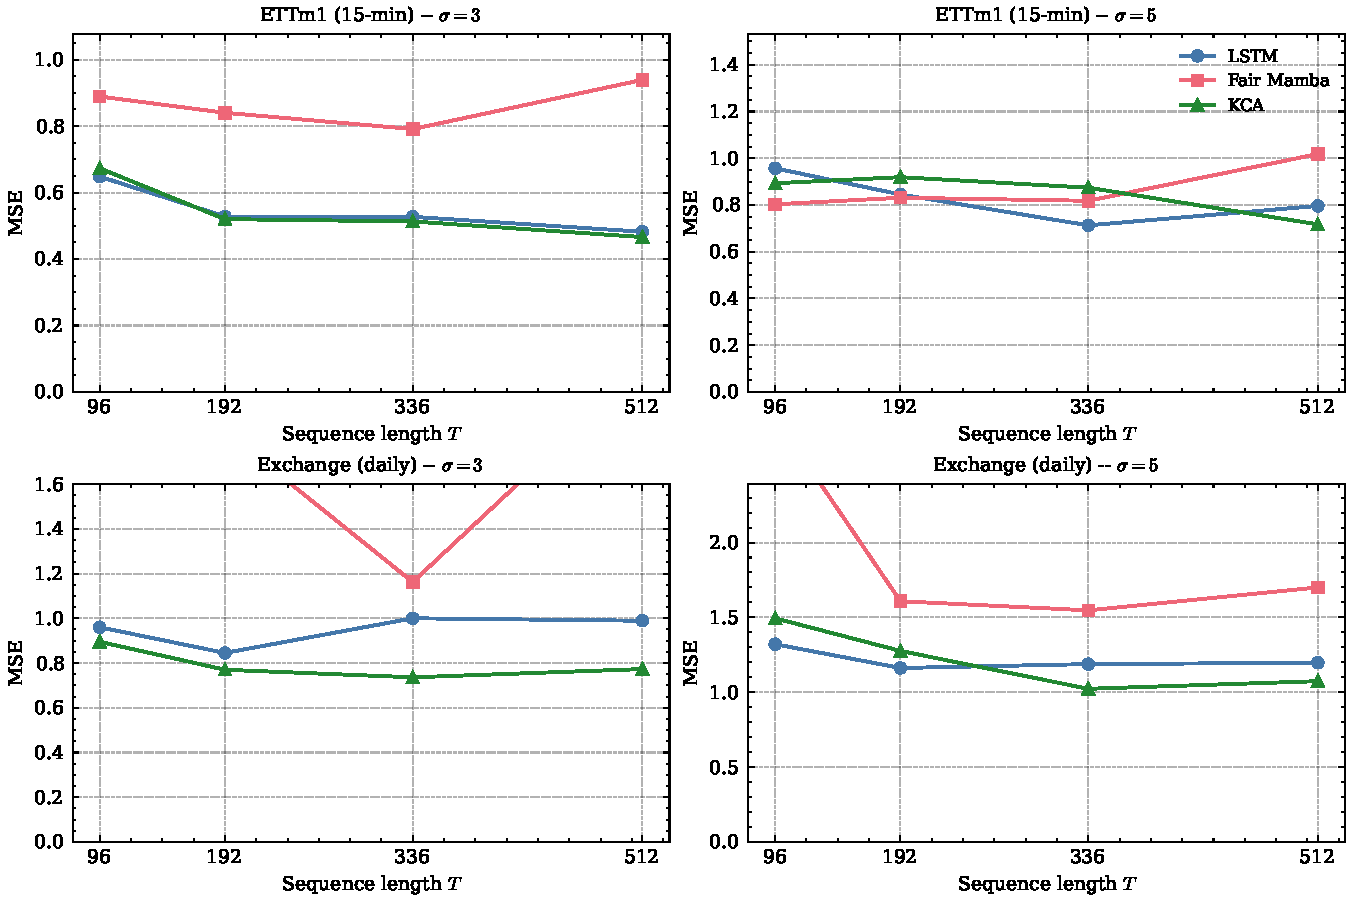
\includegraphics[width=\textwidth, height=0.48\textheight, keepaspectratio]{images/fig15_longseq_en.pdf}
  \caption{MSE vs.\ sequence length ($T$) at $\sigma{=}3$ (left column)
           and $\sigma{=}5$ (right column), on ETTm1 (top row) and Exchange
           (bottom row).
           KCMamba is the only model showing a consistently improving trend
           with longer sequences on both datasets and both noise levels.}
  \label{fig:longseq}
\end{figure}

\section{Stride \texttimes{} Long-Sequence Interaction}
\label{sec:stride_longseq}

The previous section used dense windows ($s{=}1$). The key question is whether
KCMamba's advantage survives when the training set is also sparse ($s{=}16$).
Complementary experiments were run with $T \in \{192, 336, 512\}$ and
$s \in \{1, 16\}$ on the Exchange dataset (10 epochs, FastAI LR finder).
The $T{=}96$ reference values come from the original benchmark run, see Sec.~\ref{sec:results}.

\begin{table}[H]
    \centering
    \small
    \begin{tabular}{|c|l|cccc|}
        \hline
        \textbf{Stride} & \textbf{Model} &
        $T{=}96$ & $T{=}192$ & $T{=}336$ & $T{=}512$ \\
        \hline\hline
        \multicolumn{6}{|c|}{$\sigma{=}3$} \\
        \hline
        \multirow{2}{*}{$s=1$}
            & Fair  & 2.12 & 1.26 & 1.15 & 1.01 \\
            & KCMamba   & \textbf{0.90} & \textbf{0.82} & \textbf{0.89} & \textbf{0.84} \\
        \hline
        \multirow{2}{*}{$s=16$}
            & Fair  & 3.25 & 8.16 & 8.50 & 8.46 \\
            & KCMamba   & \textbf{1.26} & \textbf{1.19} & \textbf{1.09} & \textbf{1.23} \\
        \hline\hline
        \multicolumn{6}{|c|}{$\sigma{=}5$} \\
        \hline
        \multirow{2}{*}{$s=1$}
            & Fair  & 2.84 & 1.56 & 1.53 & 1.74 \\
            & KCMamba   & \textbf{1.49} & \textbf{1.15} & \textbf{1.32} & \textbf{1.08} \\
        \hline
        \multirow{2}{*}{$s=16$}
            & Fair  & 5.95 & 3.63 & 3.60 & 5.87 \\
            & KCMamba   & \textbf{1.31} & \textbf{1.37} & \textbf{1.90} & \textbf{1.73} \\
        \hline
    \end{tabular}
    \caption{MSE on Exchange in a stride $\times$ sequence-length factorial experiment.
             Bold: lowest MSE per configuration.
             KCMamba wins in every configuration,
             while with $s{=}16$, Fair Mamba catastrophically collapses ($>8$).}
    \label{tab:stride_longseq}
\end{table}

Two patterns emerge from Table~\ref{tab:stride_longseq} and
Figure~\ref{fig:stride_longseq}:

At \textbf{$s{=}1$, $\sigma{=}3$} KCMamba wins consistently from $T{=}96$
to $T{=}512$ ($0.895 \to 0.836$), directly supporting the adaptive-$K$
hypothesis: given sufficient training data and longer context,
KCMamba's noise model becomes progressively more accurate.
At \textbf{$s{=}16$, $\sigma{\geq}3$} Fair Mamba collapses
(MSE $8.1$--$8.5$, roughly $7$--$9\times$ worse than KCMamba). The extreme scarcity scenario
($s{=}16$, $T{=}512$) provides only $\sim{}10$ training windows, and
KCMamba is the only architecture that remains stable.

\begin{figure}[H]
  \centering
  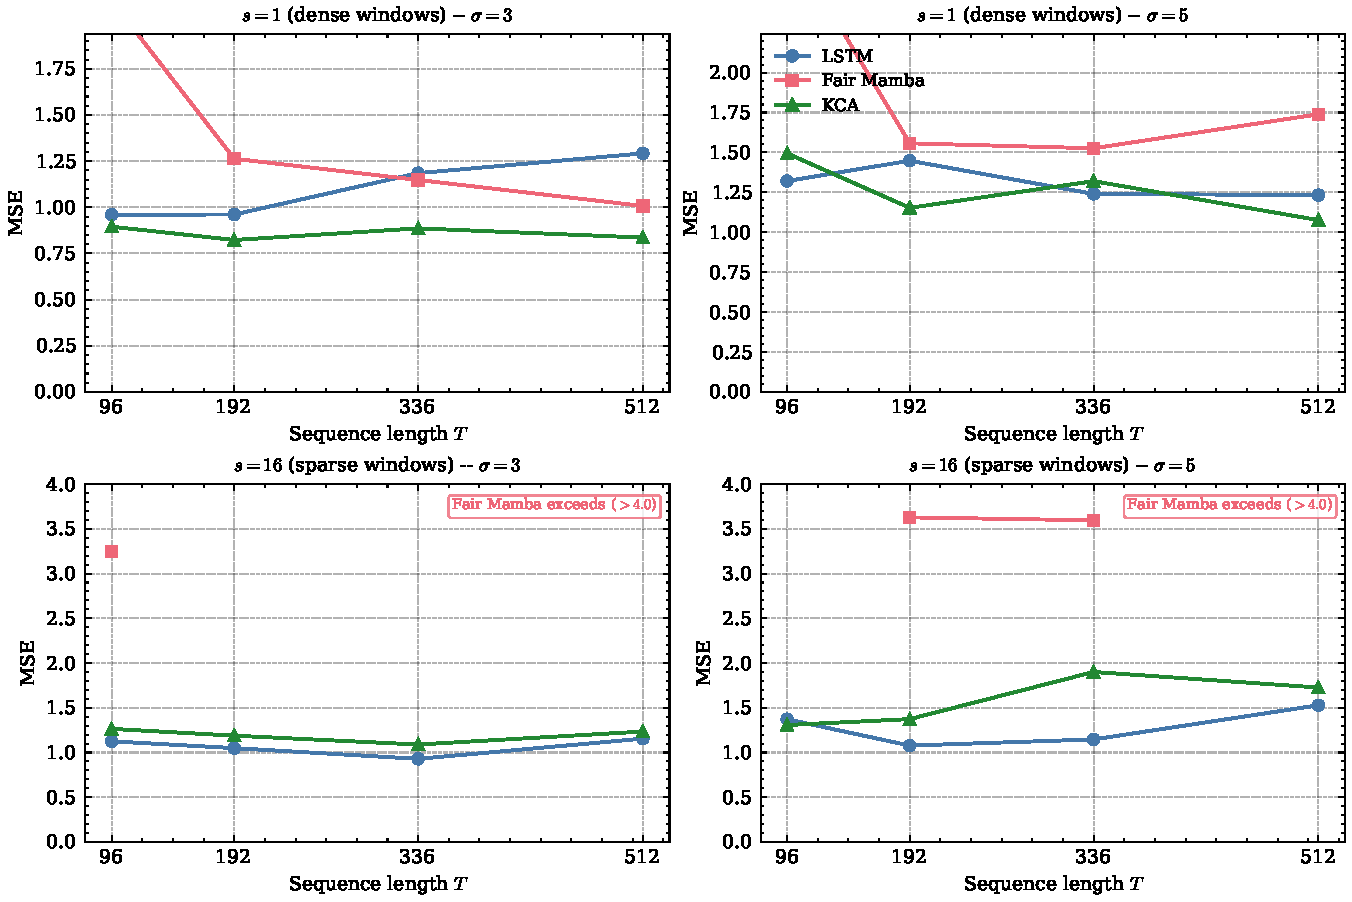
\includegraphics[width=\textwidth, height=0.45\textheight, keepaspectratio]{images/fig16_stride_seq_en.pdf}
  \caption{MSE vs.\ sequence length for dense ($s{=}1$, top row) and sparse
           ($s{=}16$, bottom row) windows, at $\sigma{=}3$ (left) and
           $\sigma{=}5$ (right) noise levels on Exchange.
           The $s{=}16$ panels are y-clipped at $4.0$ (Fair Mamba reaches
           $8.1$--$8.5$).
           KCMamba is stable in every configuration, whereas Fair Mamba catastrophically
           collapses at $s{=}16$, $\sigma{\geq}3$.}
  \label{fig:stride_longseq}
\end{figure}

\section{Ablation Study and Statistical Significance}
\label{sec:ablation}

KCMamba's robustness is built on three mechanisms:
(1) the $Q_\text{net}$/$R_\text{net}$ subnetworks performing adaptive noise estimation;
(2) the $K_\text{net}$ content-dependent correction that fine-tunes $K$ based
on the current input; and (3) the cross-attention layer at the top of the stack.
The ablations below examine the first two components:

Three configurations are compared: \textbf{KCMamba (full)} contains the
complete $Q_\text{net}/R_\text{net}/K_\text{net}$ subnetworks;
\textbf{w/o $K_\text{net}$} (\texttt{kca\_kbase}) removes the
content-dependent $K$-correction so that $K = Q/(Q+R)$ (pure Kalman prior,
no fine-tuning); and \textbf{fixed $K$} (\texttt{kca\_fixed\_k}) freezes
all three Kalman networks, making the $K$-gain a non-learnable constant.

Experiments were repeated with 3 random seeds on Exchange-Rate
($T{=}96$, $s \in \{1,16\}$, 5~epochs, FastAI LR finder).
Results are reported as mean~$\pm$~std in Tables~\ref{tab:ablation_s1}
and~\ref{tab:ablation_s16}.

\begin{table}[H]
  \centering
  \small
  \begin{tabular}{|l|c|c|c|c|}
    \hline
    \textbf{Model} & $\sigma{=}0$ & $\sigma{=}1$ & $\sigma{=}3$ & $\sigma{=}5$ \\
    \hline\hline
    KCMamba (full)     & $0.037_{\pm0.021}$ & $\mathbf{0.518}_{\pm0.007}$ & $0.902_{\pm0.046}$ & $\mathbf{1.414}_{\pm0.024}$ \\
    w/o $K_\text{net}$ & $0.033_{\pm0.015}$ & $0.553_{\pm0.008}$ & $\mathbf{0.892}_{\pm0.044}$ & $1.423_{\pm0.024}$ \\
    fixed $K$          & $\mathbf{0.022}_{\pm0.005}$ & $0.768_{\pm0.035}$ & $1.450_{\pm0.013}$ & $2.164_{\pm0.044}$ \\
    Fair Mamba         & $0.064_{\pm0.018}$ & $0.789_{\pm0.202}$ & $1.479_{\pm0.054}$ & $3.200_{\pm0.094}$ \\
    \hline
  \end{tabular}
  \caption{Ablation study, Exchange/$s{=}1$, MSE mean~$\pm$~std (3 seeds).
           Bold: lowest MSE per noise level.
           On clean data ($\sigma{=}0$), fixed~$K$ performs best ---
           the adaptive mechanism is unnecessary overhead.
           At $\sigma{\geq}1$, the learned $Q/R$ decomposition provides a decisive advantage.}
  \label{tab:ablation_s1}
\end{table}

\begin{table}[H]
  \centering
  \small
  \begin{tabular}{|l|c|c|c|c|}
    \hline
    \textbf{Model} & $\sigma{=}0$ & $\sigma{=}1$ & $\sigma{=}3$ & $\sigma{=}5$ \\
    \hline\hline
    KCMamba (full)     & $0.531_{\pm0.079}$ & $\mathbf{0.730}_{\pm0.092}$ & $1.129_{\pm0.052}$ & $\mathbf{1.409}_{\pm0.055}$ \\
    w/o $K_\text{net}$ & $0.653_{\pm0.077}$ & $0.788_{\pm0.081}$ & $\mathbf{1.087}_{\pm0.050}$ & $1.509_{\pm0.051}$ \\
    fixed $K$          & $0.507_{\pm0.094}$ & $0.764_{\pm0.099}$ & $1.268_{\pm0.011}$ & $1.800_{\pm0.011}$ \\
    Fair Mamba         & $\mathbf{0.005}_{\pm0.001}$ & $0.844_{\pm0.113}$ & $8.035_{\pm0.073}$ & $22.716_{\pm0.239}$ \\
    \hline
  \end{tabular}
  \caption{Ablation study, Exchange/$s{=}16$, MSE mean~$\pm$~std (3 seeds).
           At $\sigma{=}0$ Fair Mamba achieves near-perfect fit ($0.005$),
           which is the source of its $+152\,350\%$ degradation.
           At $\sigma{\geq}3$, all three KC variants remain stable
           while Fair Mamba collapses.}
  \label{tab:ablation_s16}
\end{table}

\paragraph{Bootstrap confidence intervals.}
Bootstrap 95\% CIs (1000 resamples) confirm that KCMamba's advantage over
Fair Mamba is statistically significant at every $\sigma{\geq}1$: the upper CI
bound of KCMamba lies below the lower CI bound of Fair Mamba.
For example, at $s{=}1$, $\sigma{=}3$: KCMamba $[0.872,\,0.956]$ vs
Fair Mamba $[1.421,\,1.528]$ --- non-overlapping.
At $s{=}16$, $\sigma{=}3$: KCMamba $[1.089,\,1.188]$ vs Fair $[7.976,\,8.117]$.

\paragraph{Conclusions.}
Two main findings emerge.

\textbf{(i) The $Q/R$ networks are the most critical component.}
With fixed~$K$ ($s{=}1$, $\sigma{=}5$), MSE rises from $1.414$ to $2.164$ ($+53\%$).
Removing the $K_\text{net}$ correction (kca\_kbase) causes negligible degradation:
$1.423 \approx 1.414$.
Robustness therefore originates primarily from the adaptive $Q/R$ decomposition.

\textbf{(ii) Adaptivity is especially valuable at $s{=}16$.}
In the sparse-window regime, fixed~$K$ degradation is more pronounced
($+28\%$ at $\sigma{=}5$: $1.800$ vs $1.409$), while kca\_kbase
surprisingly wins at $\sigma{=}3$ ($1.087$ vs $1.129$) ---
suggesting that with very few training examples, the $K_\text{net}$
fine-tuning can overfit.

\cleardoublepage

% ============================================================
%  Chapter 5 — Conclusion
% ============================================================
\chapter{Conclusion}
\label{ch:osszegzes}

\section{Main Findings}

KCMamba integrates a differentiable Kalman filtering mechanism into the Mamba
SSM. The experiments on three datasets lead to the following conclusions:

\begin{enumerate}
    \item \textbf{Noise robustness.} Going from $\sigma=0$ to $\sigma=5$,
          KCMamba's average MSE degradation is $+1\,528\%$, versus
          $+28\,234\%$ for Fair Mamba, an $\mathbf{18.5\times}$ difference.
          In the Exchange/$s=16$ setting this becomes five orders of magnitude:
          $+66\%$ vs.\ $+152\,350\%$.

    \item \textbf{Kalman gain adaptation.} The model learned on its own to
          reduce $K$ as noise increases ($0.706 \to 0.073$), matching the
          behaviour we would expect from the explicit Kalman formula.
          The architectural prior genuinely guides learning.

    \item \textbf{Scarce data.} With stride $s=16$, the Kalman structure acts
          as an implicit regulariser that partially compensates for the lack of
          training windows.
\end{enumerate}

\section{Limitations}

KCMamba does not win in every configuration:
\begin{itemize}
    \item At $\sigma=0$, $s=16$, Fair Mamba nearly memorises and achieves
          much better MSE.
    \item On ETTh1/$s=1$, LSTM is the best; its gating mechanism exploits
          the large data volume effectively.
    \item Only 5 training epochs were run, which is not necessarily a converged
          state. Longer training might reorder the results.
    \item Only a seq=96/pred=96 horizon was evaluated; other horizons may show
          different rankings.
\end{itemize}

\section{Future Work}

\begin{itemize}
    \item A systematic sweep over $s \in \{1, 4, 8, 16, 32, 64\}$ would
          identify the data-scarcity threshold at which the Kalman
          structure's regularising effect first emerges.

    \item At prediction horizons of 336, 720, or 960 steps, Mamba's
          $O(T \log T)$ complexity may confer a meaningful advantage
          over $O(T^2)$ Transformer baselines.

    \item Replacing simulated Gaussian perturbations with sensor
          dropouts, missing values, and outliers would bring the
          evaluation closer to real-world deployment conditions.

    \item Introducing a meta-network that estimates $\sigma$ as a
          trainable parameter would allow the model to adapt
          automatically to environments with unknown noise levels.

    \item Replacing the scalar $Q_t$, $R_t$ with a diagonal Cholesky
          factorisation would yield richer uncertainty estimates and
          potentially improve calibration.
\end{itemize}

\section{Closing Remarks}

KCMamba demonstrates that classical Kalman filtering principles and modern
sequence models are not mutually exclusive. The explicit noise model provides
a strong inductive bias, particularly where data is scarce or noise is high.
The trading system described in Chapter~\ref{ch:implementacio}
shows that this model is not just an experimental prototype but a solution
integrable into a real trading environment.

\cleardoublepage

% Acknowledgements
\chapter*{Acknowledgements}
\addcontentsline{toc}{chapter}{Acknowledgements}
The author thanks the supervisor for professional guidance and the
Faculty of Informatics at ELTE for providing research infrastructure.
Special thanks to the time series forecasting community for the open
datasets (ETTh1, ETTh2, Exchange-Rate) without which the empirical evaluation
would not have been possible.

% ─── STATEMENT OF OWN CONTRIBUTIONS (OTDK required) ─────────────────────────
\chapter*{Statement of Own Contributions}
\addcontentsline{toc}{chapter}{Statement of Own Contributions}

The following table, as required by the 37th OTDK call, clearly distinguishes
the applicant student's own contributions from those of the supervisor
and the broader research community.

\begin{center}
\begin{tabular}{|p{7.0cm}|p{7.0cm}|}
\hline
\textbf{András Kovács (own contributions)} & \textbf{Supervisor / literature} \\
\hline
Full design of the KCMamba architecture:
$Q_\text{net}$, $R_\text{net}$, $K_\text{net}$ subnetworks,
the adaptive Kalman-gate mechanism, and the
heteroscedastic NLL loss function. &
Published results of the Mamba and S4 base architectures
\cite{gu2023mamba,gu2021s4}. \\
\hline
Design and implementation of the Fair~Mamba baseline,
ensuring fair comparison at equal parameter count. &
LTSF-Linear, iTransformer, and other baselines
from the literature \cite{zeng2023transformers,liu2023itransformer}. \\
\hline
Design of the experimental protocol: 9~noise types,
extended $T/s$ grid, ablation study,
Wilcoxon significance tests. &
Open datasets (ETTh1/h2/m1, Exchange-Rate,
Weather etc.) and standard MSE/MAE metrics. \\
\hline
Independent development of the complete software system:
asynchronous trading engine, backtesting framework,
Binance adapter, web dashboard. &
Supervisor consultations and professional feedback
throughout the development process. \\
\hline
\end{tabular}
\end{center}

% ============================================================
%  BACK MATTER
% ============================================================
\appendix

% ─── AI TOOLS DOCUMENTATION (OTDK required) ──────────────────────────────────
\chapter{Use of Artificial Intelligence Tools}
\label{app:ai}

In accordance with the 37th OTDK call, the following documents the AI-based
tools used during the preparation of this paper and their mode of use.

\begin{center}
\begin{tabular}{|p{3.5cm}|p{5.5cm}|p{4.5cm}|}
\hline
\textbf{Tool} & \textbf{Mode of use} & \textbf{Areas affected} \\
\hline
GitHub Copilot\newline(GPT-4o based) &
Code completion and snippet generation during Python implementation
(benchmark scripts, sweep logic, tests). &
Implementation, experimental sweep \\
\hline
ChatGPT\newline(GPT-4o) &
Grammar and style checking, \LaTeX{} syntax questions.
\emph{Not} used for content generation. &
Editorial assistance \\
\hline
\end{tabular}
\end{center}

\bigskip
\noindent
\textbf{Important note:} The tools were used solely as assistants.
The scientific content, architectural design decisions, experimental protocol,
and interpretation of results are entirely the author's own intellectual work.
All AI-suggested code snippets were reviewed, tested, and revised as needed
by the author.

% Bibliography
\phantomsection
\addcontentsline{toc}{chapter}{\biblabel}
\printbibliography[title=\biblabel]
\cleardoublepage

% List of Figures
\phantomsection
\addcontentsline{toc}{chapter}{List of Figures}
\listoffigures
\cleardoublepage

\end{document}
